\section{Experimental Evaluation}
\label{sec:experiments}

\rtag{E4, R1.5, R2.5}\begin{revblock}The evaluation combines real and simulated components. The clinical data (WDBC~\cite{wolberg1995breast}) and the learning computation are real: every reported accuracy results from training the stated model on the stated data, and the server run times are measured on the released code. The client partition, the devices and batteries, the wireless channel and the adversaries are simulated, and the energy is computed from the models of Section~\ref{sec:model}; no energy figure in this article was measured on hardware. The physiological streams used to exercise the twin layer are synthetic. The evaluation therefore characterizes the behaviour of the scheduling and aggregation rules under the stated models; hardware measurements and clinical validation are outside its scope.\end{revblock}

\rtag{R1.7(3), R1.7(4)}\begin{revblock}The WDBC data set contains 569 cases, 212 malignant and 357 benign, each described by 30 real-valued features computed from a digitized image of a fine-needle aspirate of a breast mass~\cite{wolberg1995breast}. It is loaded from the scikit-learn library; the positive class is malignant. A stratified split with a fixed seed assigns 80\% of the cases to training and 20\% to testing, and 10\% of the training part is held out for validation, which gives \V{ntrain} training, \V{nval} validation and \V{ntest} test cases. The features are standardized with the statistics of the training part.\end{revblock}

\subsection{Compared Methods}
\label{subsec:methods}
The proposed ATEF-DT is compared with the following methods.

\begin{itemize}
	\item \rtag{E4, R2.4}\begin{revblock}\textbf{FedAvg-Full}~\cite{mcmahan2017communication} lets every reachable client take part in every round, without a budget, at full precision and with the weights of~\eqref{eq:fedavg}. It is the reference for accuracy and an upper reference for energy.\end{revblock}

	\item \rtag{E4, R2.4}\begin{revblock}\textbf{FedAvg-Random}~\cite{mcmahan2017communication} draws $S_{\max}$ clients uniformly at random, without replacement, from the reachable clients of the round and aggregates at full precision with~\eqref{eq:fedavg}. The participation count of a client after $R$ rounds has mean $Rq$ and variance $Rq(1-q)$ with $q=S_{\max}/P$, so the expected Jain index is approximately
	\begin{equation}
		\E[J]\approx\frac{Rq}{Rq+1-q}=\V{jainexp}\qquad(R=50,\;q=0.4).
		\label{eq:jainexp}
	\end{equation}
	A value far below this would indicate an implementation that does not sample uniformly.\end{revblock}

	\item \textbf{EA-FL}~\cite{nishio2019client,arouj2022towards} is energy-greedy selection: the $S_{\max}$ feasible clients with the smallest predicted energy, an instantaneous battery test, full precision and~\eqref{eq:fedavg}. It represents energy-driven selection and is not a re-implementation of a particular system.

	\item \textbf{FairFedCS}~\cite{shi2023fairfedcs} selects the clients with the largest index $\sigma r_p+Q_p$, where $r_p=(a_p+1)/(a_p+b_p+2)$ is a Beta reputation and $Q_p$ is a fairness queue that grows by $(S_{\max}/P)\,r_p$ when the client is not selected and decreases by one when it is ($\sigma=0.6$). The contribution of a client is the leave-one-out change of the validation loss, a simplification of the Shapley-value estimate of~\cite{shi2023fairfedcs}.

	\item \textbf{Energy+Trust} combines energy-greedy selection with the credibility engine of Section~\ref{subsec:credibility}. \rtag{R1.1}\rev{It stands for the combination of energy-aware scheduling and trust-weighted aggregation of which Trust-FedGNN~\cite{reis2026trustfedgnn} is an instance, without the graph neural model of that work, which has no counterpart for tabular data.}

	\item \textbf{Energy+Fair} uses the score~\eqref{eq:score} with $\lambda_T=0$, the twin screen, full precision and~\eqref{eq:fedavg}.

	\item \rtag{E1, R1.1, R2.1}\begin{revblock}\textbf{Weighted sum} ranks the clients by $\lambda_E\tilde e_p+\lambda_F\tilde u_p+\lambda_T\tilde t_p$. This and the next two rules keep the feasibility screen, the quantizer, the credibility engine and the aggregation rule of ATEF-DT, so that only the selection rule differs.\end{revblock}

	\item \rtag{E1, R1.1, R2.1}\begin{revblock}\textbf{Drift-plus-penalty}~\cite{huang2021efficiency} keeps a virtual queue $Z_p\leftarrow\max\{0,Z_p+S_{\max}/P-\mathbb{1}[p\in\cS^{(r)}]\}$ and selects the clients with the largest $Z_p-V\tilde e_p$, following the Lyapunov construction of RBCS-F with the energy factor as the penalty.\end{revblock}

	\item \rtag{E1, R1.1, R2.1}\begin{revblock}\textbf{Seq-EF} and \textbf{Seq-FE} are two-stage pipelines: Seq-EF keeps the $\bar k$ feasible clients with the smallest $\tilde e_p$ and selects among them by $\tilde u_p$, and Seq-FE reverses the order.\end{revblock}

	\item \textbf{Robust aggregation rules}: the coordinate-wise median, the trimmed mean with 20\% trimmed on each side~\cite{yin2018byzantine}, Multi-Krum~\cite{blanchard2017machine} and the geometric median~\cite{pillutla2022robust}, run with uniform selection at full precision.

	\item \textbf{Matched variants} keep the selection, screen and quantizer of ATEF-DT and remove the reputation layer ($\lambda_T=0$, no gate); the accepted updates are clipped and combined by an unweighted mean or by a geometric median.
\end{itemize}

\subsection{Implementation Details}
\label{subsec:implementation}
\rtag{R1.7(3)}\rev{The training cases are divided among the $P=20$ clients by a Dirichlet partition with concentration $0.5$ over the two classes~\cite{hsu2019measuring}, which produces unequal sizes and label skew; a draw is repeated until every client holds at least six cases, and over the \V{nseeds} seeds the client sizes range from \V{npmin} to \V{npmax}.} The model is a perceptron with one hidden layer of 64 rectified-linear units and a logistic output ($d=\V{d}$ parameters), trained with the cross-entropy loss. Each selected client performs one full-batch gradient step per round ($E=1$), so that a round with FedAvg weights is one step of federated gradient descent. \rtag{E5, R2.7}\rev{The learning rate was selected on the validation split, with FedAvg-Full and not with the proposed method, from $\{0.1,0.2,0.5,1.0\}$; the mean validation losses were \V{lrval-01}, \V{lrval-02}, \V{lrval-05} and \V{lrval-10}, and $\eta=\V{lr}$ was retained for all methods.} \rtag{E5, R2.7}\rev{ATEF-DT and all compared methods are implemented in Python with NumPy, SciPy and scikit-learn; the complete protocol runs in about three minutes on one processor core.}

Table~\ref{tab:setup} lists all implementation and simulation parameters. A seed fixes the partition, the initial model, the device parameters, the complete fading sequence and the placement of the adversaries, and these are identical for all methods run with that seed, so that methods are compared on common random numbers. All results refer to WDBC and are means over \V{nseeds} seeds (0 to 4); tables report mean\,$\pm$\,sample standard deviation. With the outage rule of Section~\ref{subsec:energy}, a device is unreachable in \V{outage}\% of the client-rounds. The batteries of Table~\ref{tab:setup} are large relative to the consumption of 50 rounds, so the reserve is never approached in the experiments of Sections~\ref{subsec:accuracy}--\ref{subsec:byzantine} (\V{below-main} clients below the reserve across all methods and seeds); the feasibility screen and the twin are exercised separately, with small batteries, in a functional test reported in Table~\ref{tab:twin}.

\begin{table}[t]
	\centering
	\revcap{E5}{Implementation and simulation parameters.}
	\label{tab:setup}
	\footnotesize
	\setlength{\tabcolsep}{3pt}
	\begin{tabularx}{\columnwidth}{>{\raggedright\arraybackslash}X l}
		\toprule
		\textbf{Parameter} & \textbf{Value} \\
		\midrule
		Clients $P$; budget $S_{\max}$; rounds $R$ & 20; 8; 50 \\
		Local passes $E$; learning rate $\eta$ & 1; \V{lr} \\
		Computation factor $\kappa_p$ & uniform on $[0.5,2]$ \\
		Initial battery $C_p^{(0)}$ & uniform on $[80,200]$ J \\
		Reserve $C_{\mathrm{res}}$; reference level $C_{\mathrm{ref}}$ & 10 J; 20 J \\
		Computation energy coefficient $\alpha$ & $10^{-6}$ J \\
		Transmit power $P_{\mathrm{tx}}$; amplifier efficiency $\eta_{\mathrm{PA}}$ & 0.1 W; 0.35 \\
		Packet error rate $\varepsilon_{\mathrm{PER}}$; overhead $\nu$ & $10^{-2}$; 0.15 \\
		Bandwidth $W$; noise term $\sigma^2W\Gamma$ & 1 MHz; $10^{-3}$ W \\
		Mean channel gain $\bar h_p$ & exponential, mean 1 \\
		Outage threshold $\vartheta_{\min}$ & 1 bit/s/Hz \\
		Base-station power $P_{\mathrm{BS}}$; receive power $P_{\mathrm{rx}}$ & 1 W; 50 mW \\
		Bit-widths $b_{\min}$, $b_{\max}$; exponent $\gamma_b$; metadata $c_q$ & 4, 16; 0.5; 64 bit \\
		Forgetting factor $\mu$; threshold $\rho_{\min}$ & 0.6; 0.05 \\
		Weiszfeld tolerance; iteration limit & $10^{-5}$; 200 \\
		Exponents $(\lambda_E,\lambda_F,\lambda_T)$; offset $\varepsilon_0$ & $(1.0,\,3.0,\,0.4)$; 0.1 \\
		\bottomrule
	\end{tabularx}
\end{table}

Accuracy, sensitivity (recall of the malignant class) and specificity are measured on the whole test set after the last round. Energy is the device energy of Section~\ref{subsec:energy}, summed over clients and rounds and split into computation, uplink, downlink reception and signalling. Participation fairness is the Jain index of the selection counts over all $P$ clients. Traffic is counted in bits on the uplink, the downlink and for the state reports. Under attack, four quantities describe the reputation layer: the share of selections that go to adversaries after the attack starts, the share of the aggregation coefficients $\beta_p^{(r)}$ carried by their updates, the fraction of received malicious updates that are rejected, and the number of adversaries barred; the honest false-exclusion rate is the fraction of honest clients whose reputation falls below $\rho_{\min}$. The success rate of the backdoor is the fraction of malignant test cases that are classified as benign when the trigger is applied. Differences between methods are tested with a paired $t$-test over the seeds. With \V{nseeds} seeds such a test has little power, and a non-significant difference is not evidence of equivalence.

\FloatBarrier
\section{Results and Discussion}
\label{sec:results}
This section reports the results in the order of the evaluation: accuracy and convergence, energy and traffic, participation fairness, the comparison with alternative multi-objective schedulers, robustness to Byzantine clients together with the functional test of the twin layer, the ablation, scalability and sensitivity to the energy parameters. It closes with the limitations of the study.

\subsection{Accuracy and Convergence}
\label{subsec:accuracy}
Table~\ref{tab:main} and Figure~\ref{fig:convergence} report the comparison without adversaries. ATEF-DT reaches \Vpm{acc-atef}{accsd-atef}\% against \Vpm{acc-full}{accsd-full}\% for FedAvg-Full and \Vpm{acc-rand}{accsd-rand}\% for FedAvg-Random. The difference of \V{accgap-full} percentage points to FedAvg-Full is not significant ($p=\V{p-atef}$). Energy-greedy selection is less accurate (\V{acc-eafl}\% for EA-FL), because it trains on the data of a small fixed subset of clients. \rtag{R1.5}\rev{The accuracy of ATEF-DT is not uniform across the classes: its sensitivity is \V{sens-atef}\%, \V{sensgap-full} points below that of FedAvg-Full, while its specificity is higher. On the \V{ntest} test cases this corresponds to about one additional missed malignant case, and the difference is not significant over \V{nseeds} seeds ($p=\V{p-sens-atef}$), but the direction is the clinically less favourable one and is listed among the limitations.} In Figure~\ref{fig:convergence}(a) the test loss of ATEF-DT settles above that of the FedAvg variants (\V{loss-atef} against \V{loss-full} for FedAvg-Full). This is the cost of the aggregation rule: the step scale $s^{(r)}$ is below one (Section~\ref{subsec:fairres}) and the weights follow reputation and not data volume.

\begin{table*}[t]
	\centering
	\revcap{R1.5}{Performance on WDBC without adversaries after 50 rounds ($p$: paired $t$-test of accuracy against FedAvg-Full).}
	\label{tab:main}
	\footnotesize
	\begin{tabular*}{\linewidth}{@{\extracolsep{\fill}}lccccccc}
		\toprule
		\textbf{Method} & \textbf{Accuracy (\%)} & \textbf{Sensitivity (\%)} & \textbf{Specificity (\%)} & \textbf{Energy (J)} & \textbf{Jain index} & \textbf{Transmissions} & $\boldsymbol{p}$ \\
		\midrule
		\tabin{tab_main}
		\bottomrule
	\end{tabular*}
\end{table*}

\begin{figure*}[t]
	\centering
	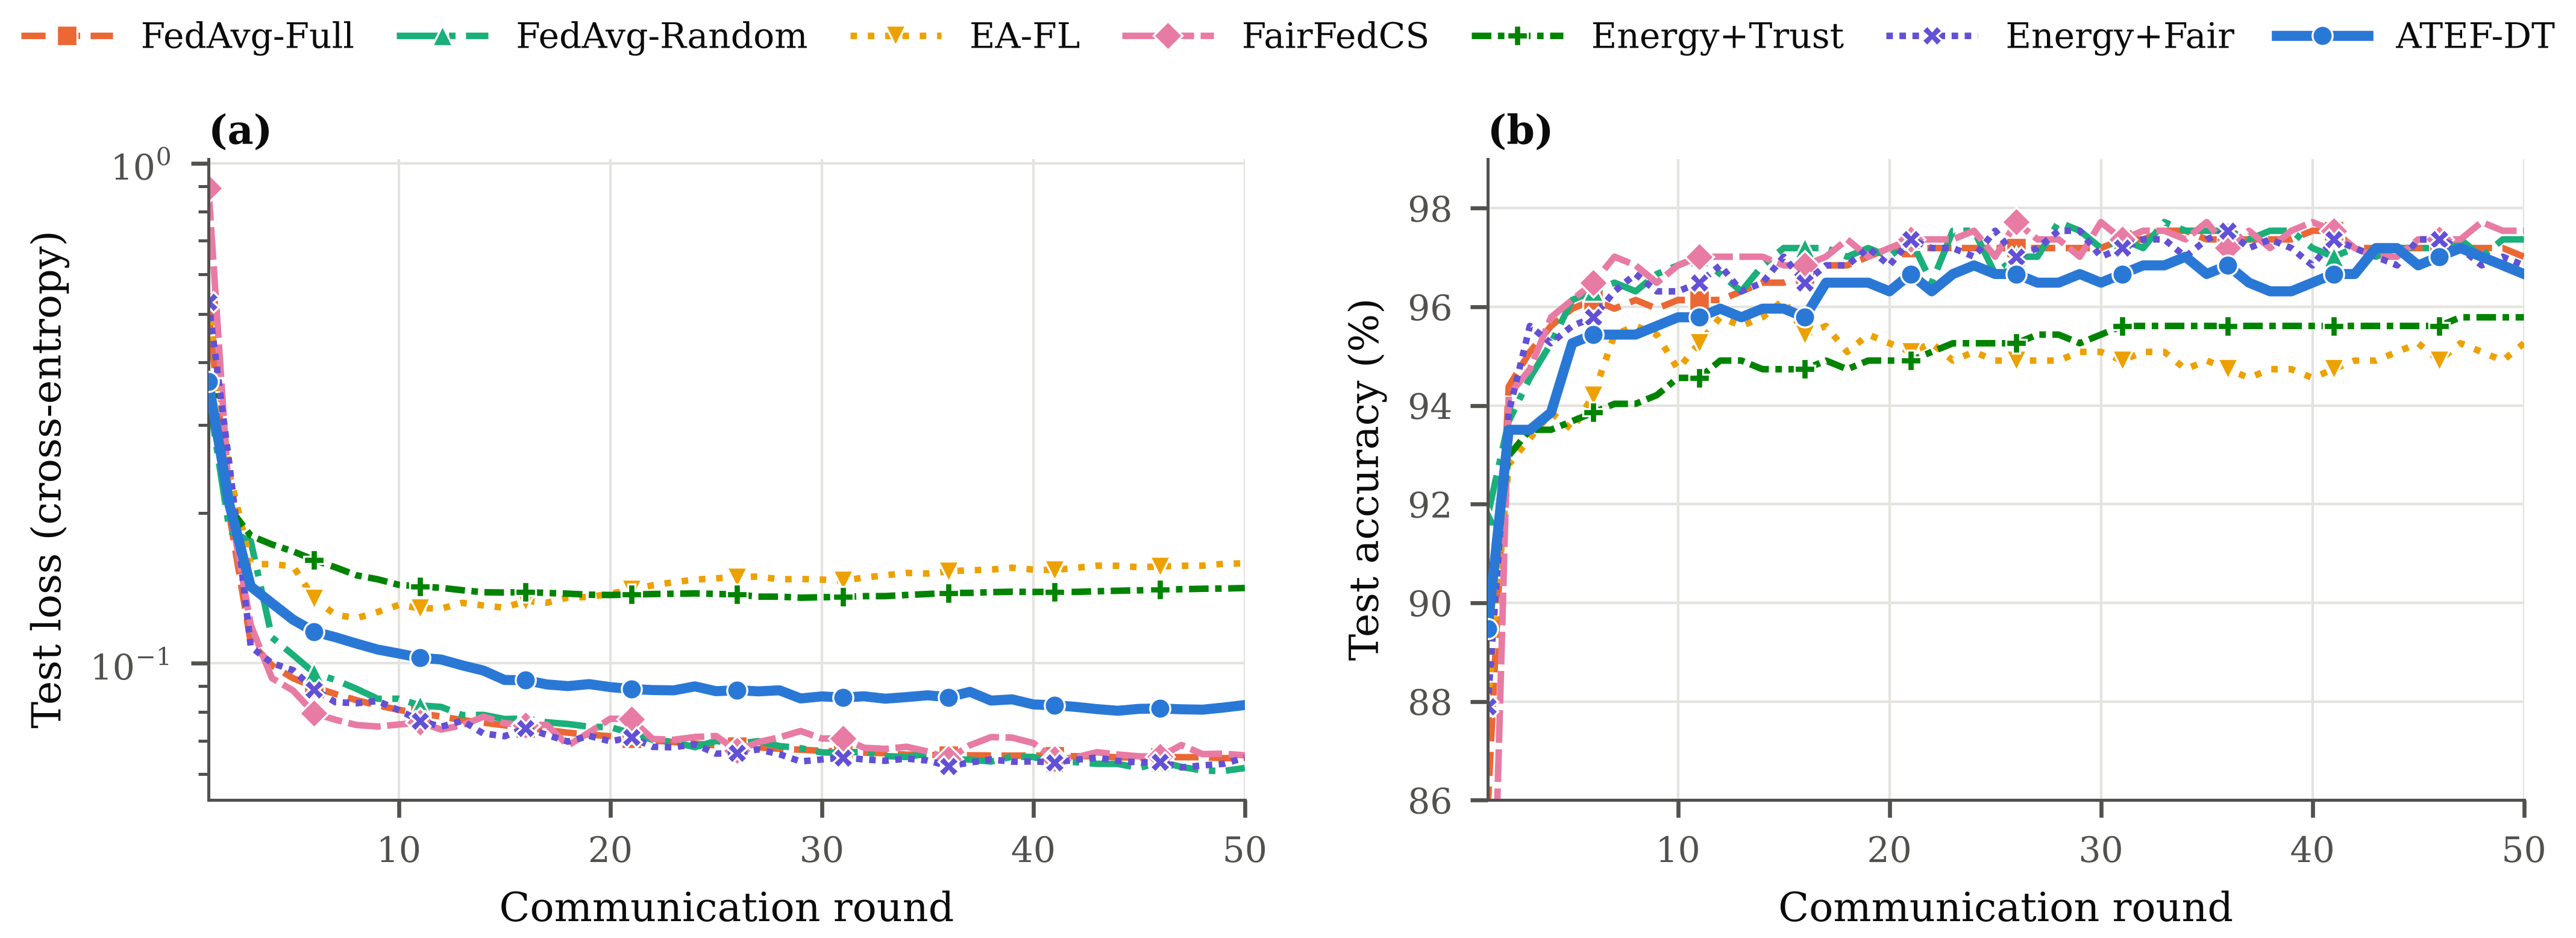
\includegraphics[width=\textwidth]{figures/fig_convergence}
	\revcap{R1.7(5), R1.7(6)}{Convergence on WDBC: (a)~test loss and (b)~test accuracy.}
	\label{fig:convergence}
\end{figure*}

\subsection{Energy and Traffic}
\label{subsec:energyres}
\rtag{R1.5}\begin{revblock}Table~\ref{tab:energy} and Figure~\ref{fig:energy} give the energy accounts. ATEF-DT consumes \Vpm{E-atef}{Esd-atef}~J. This is \V{sav-full}\% less than FedAvg-Full (\V{E-full}~J) and \V{sav-rand}\% less than FedAvg-Random (\V{E-rand}~J; paired $p=\V{p-E-atef-rand}$). The two figures answer different questions. FedAvg-Full has no budget and makes \V{tx-full} transmissions against 400, so most of the first saving is the effect of selecting eight clients per round: FedAvg-Random already saves \V{sav-rand-full}\% relative to FedAvg-Full. The comparison at equal budget is the one with FedAvg-Random. Of the \V{sav-rand}\% saved there, \V{Ecomp-sav-rand}~J come from computation, because the score prefers inexpensive clients among those that are under-served, and \V{Eul-sav-rand}~J from the uplink, because of quantization. EA-FL remains the least energy-consuming method at \V{E-eafl}~J. ATEF-DT spends \V{extra-eafl}\% more, which is the cost of spreading participation across clients; Section~\ref{subsec:fairres} shows what this buys in fairness.

\begin{table*}[t]
	\centering
	\revcap{R1.5}{Device energy (J) over 50 rounds and saving relative to FedAvg-Full and FedAvg-Random.}
	\label{tab:energy}
	\footnotesize
	\begin{tabular*}{\linewidth}{@{\extracolsep{\fill}}lccccccc}
		\toprule
		\textbf{Method} & \textbf{Computation} & \textbf{Uplink} & \textbf{Downlink} & \textbf{Signalling} & \textbf{Total} & \textbf{vs.\ Full (\%)} & \textbf{vs.\ Random (\%)} \\
		\midrule
		\tabin{tab_energy}
		\bottomrule
	\end{tabular*}
\end{table*}

\begin{figure*}[t]
	\centering
	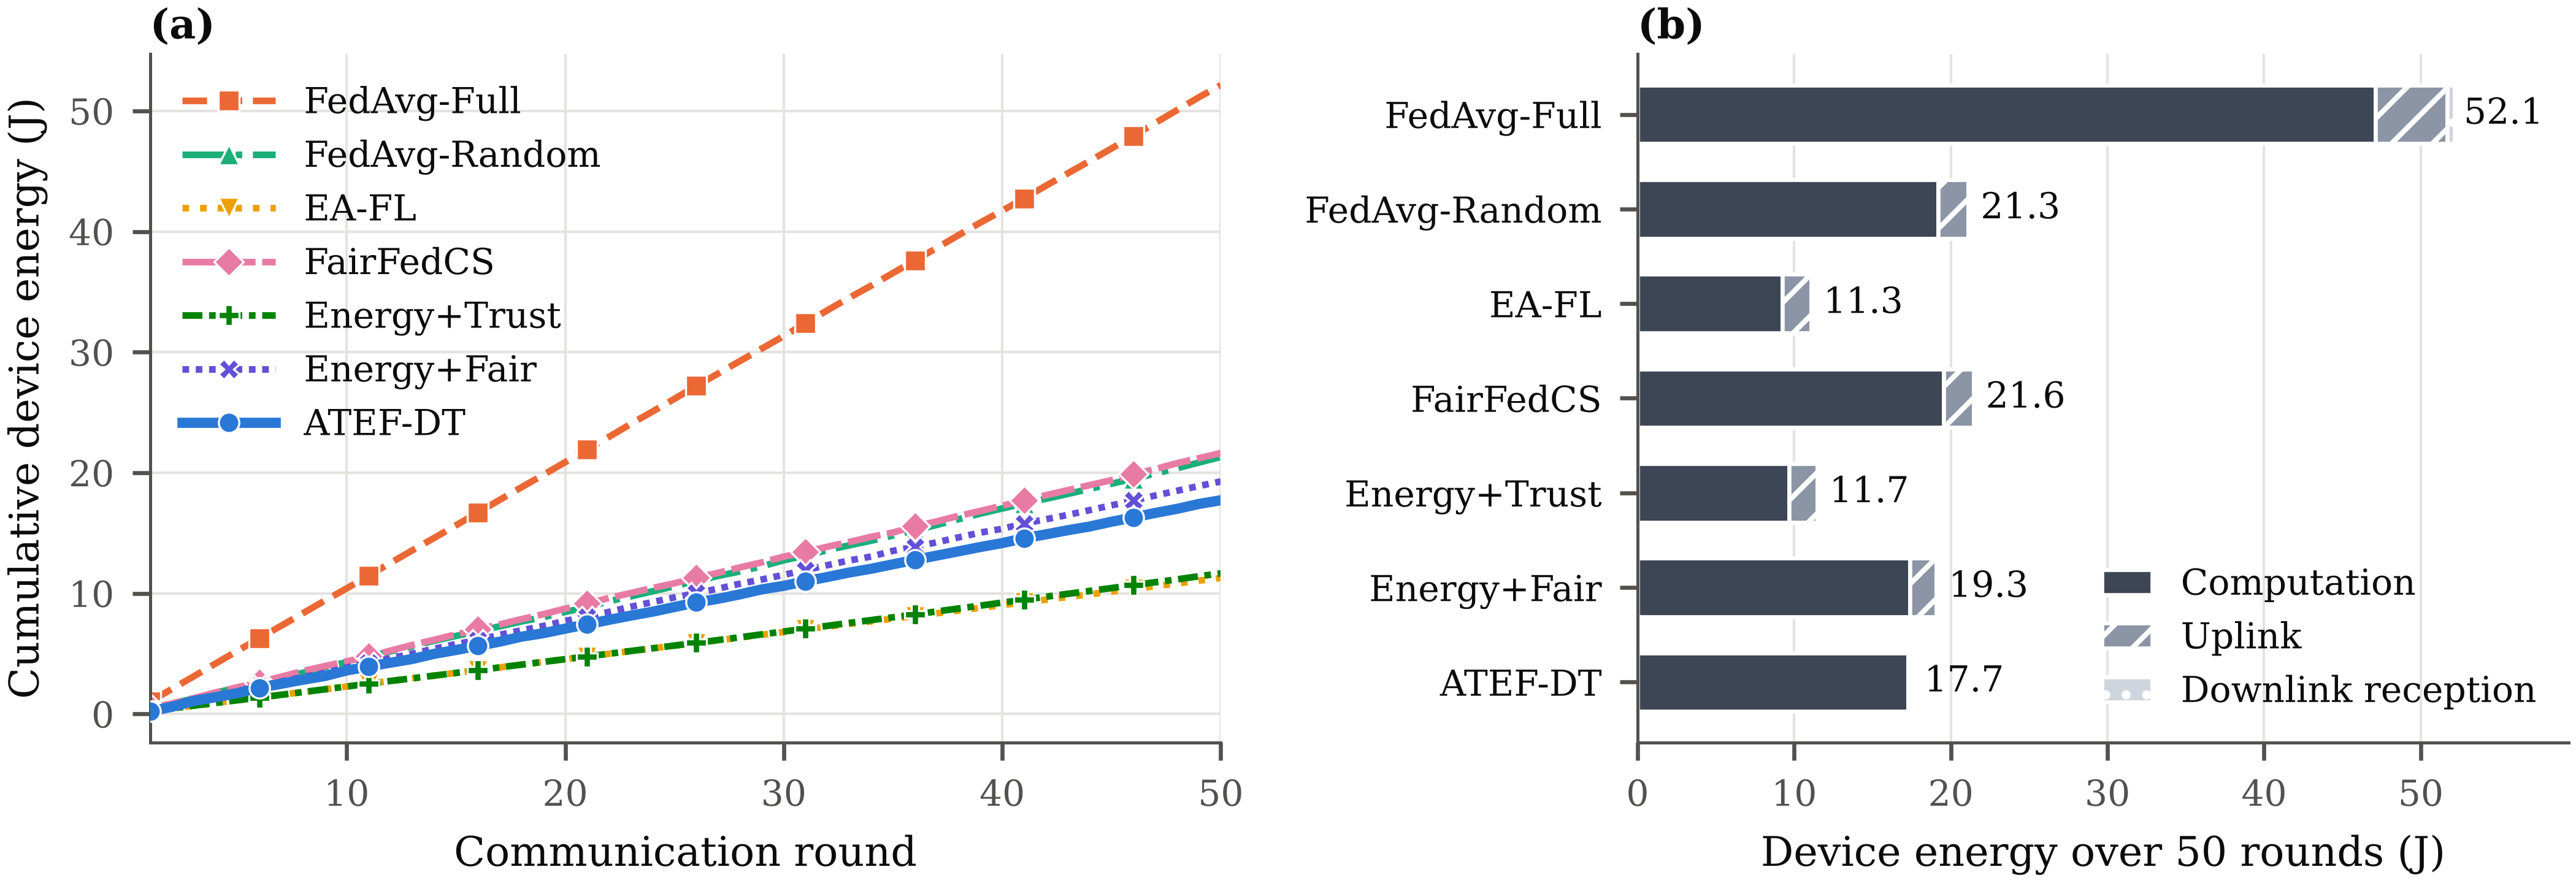
\includegraphics[width=\textwidth]{figures/fig_energy}
	\revcap{R1.5, R1.7(6)}{Device energy: (a)~cumulative energy and (b)~energy composition after 50 rounds.}
	\label{fig:energy}
\end{figure*}

\begin{table*}[t]
	\centering
	\revcap{R1.5}{Uplink traffic and energy of the bit-width policies under the ATEF-DT selection rule.}
	\label{tab:volume}
	\footnotesize
	\begin{tabular*}{\linewidth}{@{\extracolsep{\fill}}lccccccc}
		\toprule
		\textbf{Policy} & \textbf{Mean bits} & \textbf{Payload (Mb)} & \textbf{Metadata (Mb)} & \textbf{Uplink (Mb)} & \textbf{Reduction} & \textbf{Uplink energy (J)} & \textbf{Accuracy (\%)} \\
		\midrule
		\tabin{tab_volume}
		\bottomrule
	\end{tabular*}
\end{table*}

\begin{figure}[t]
	\centering
	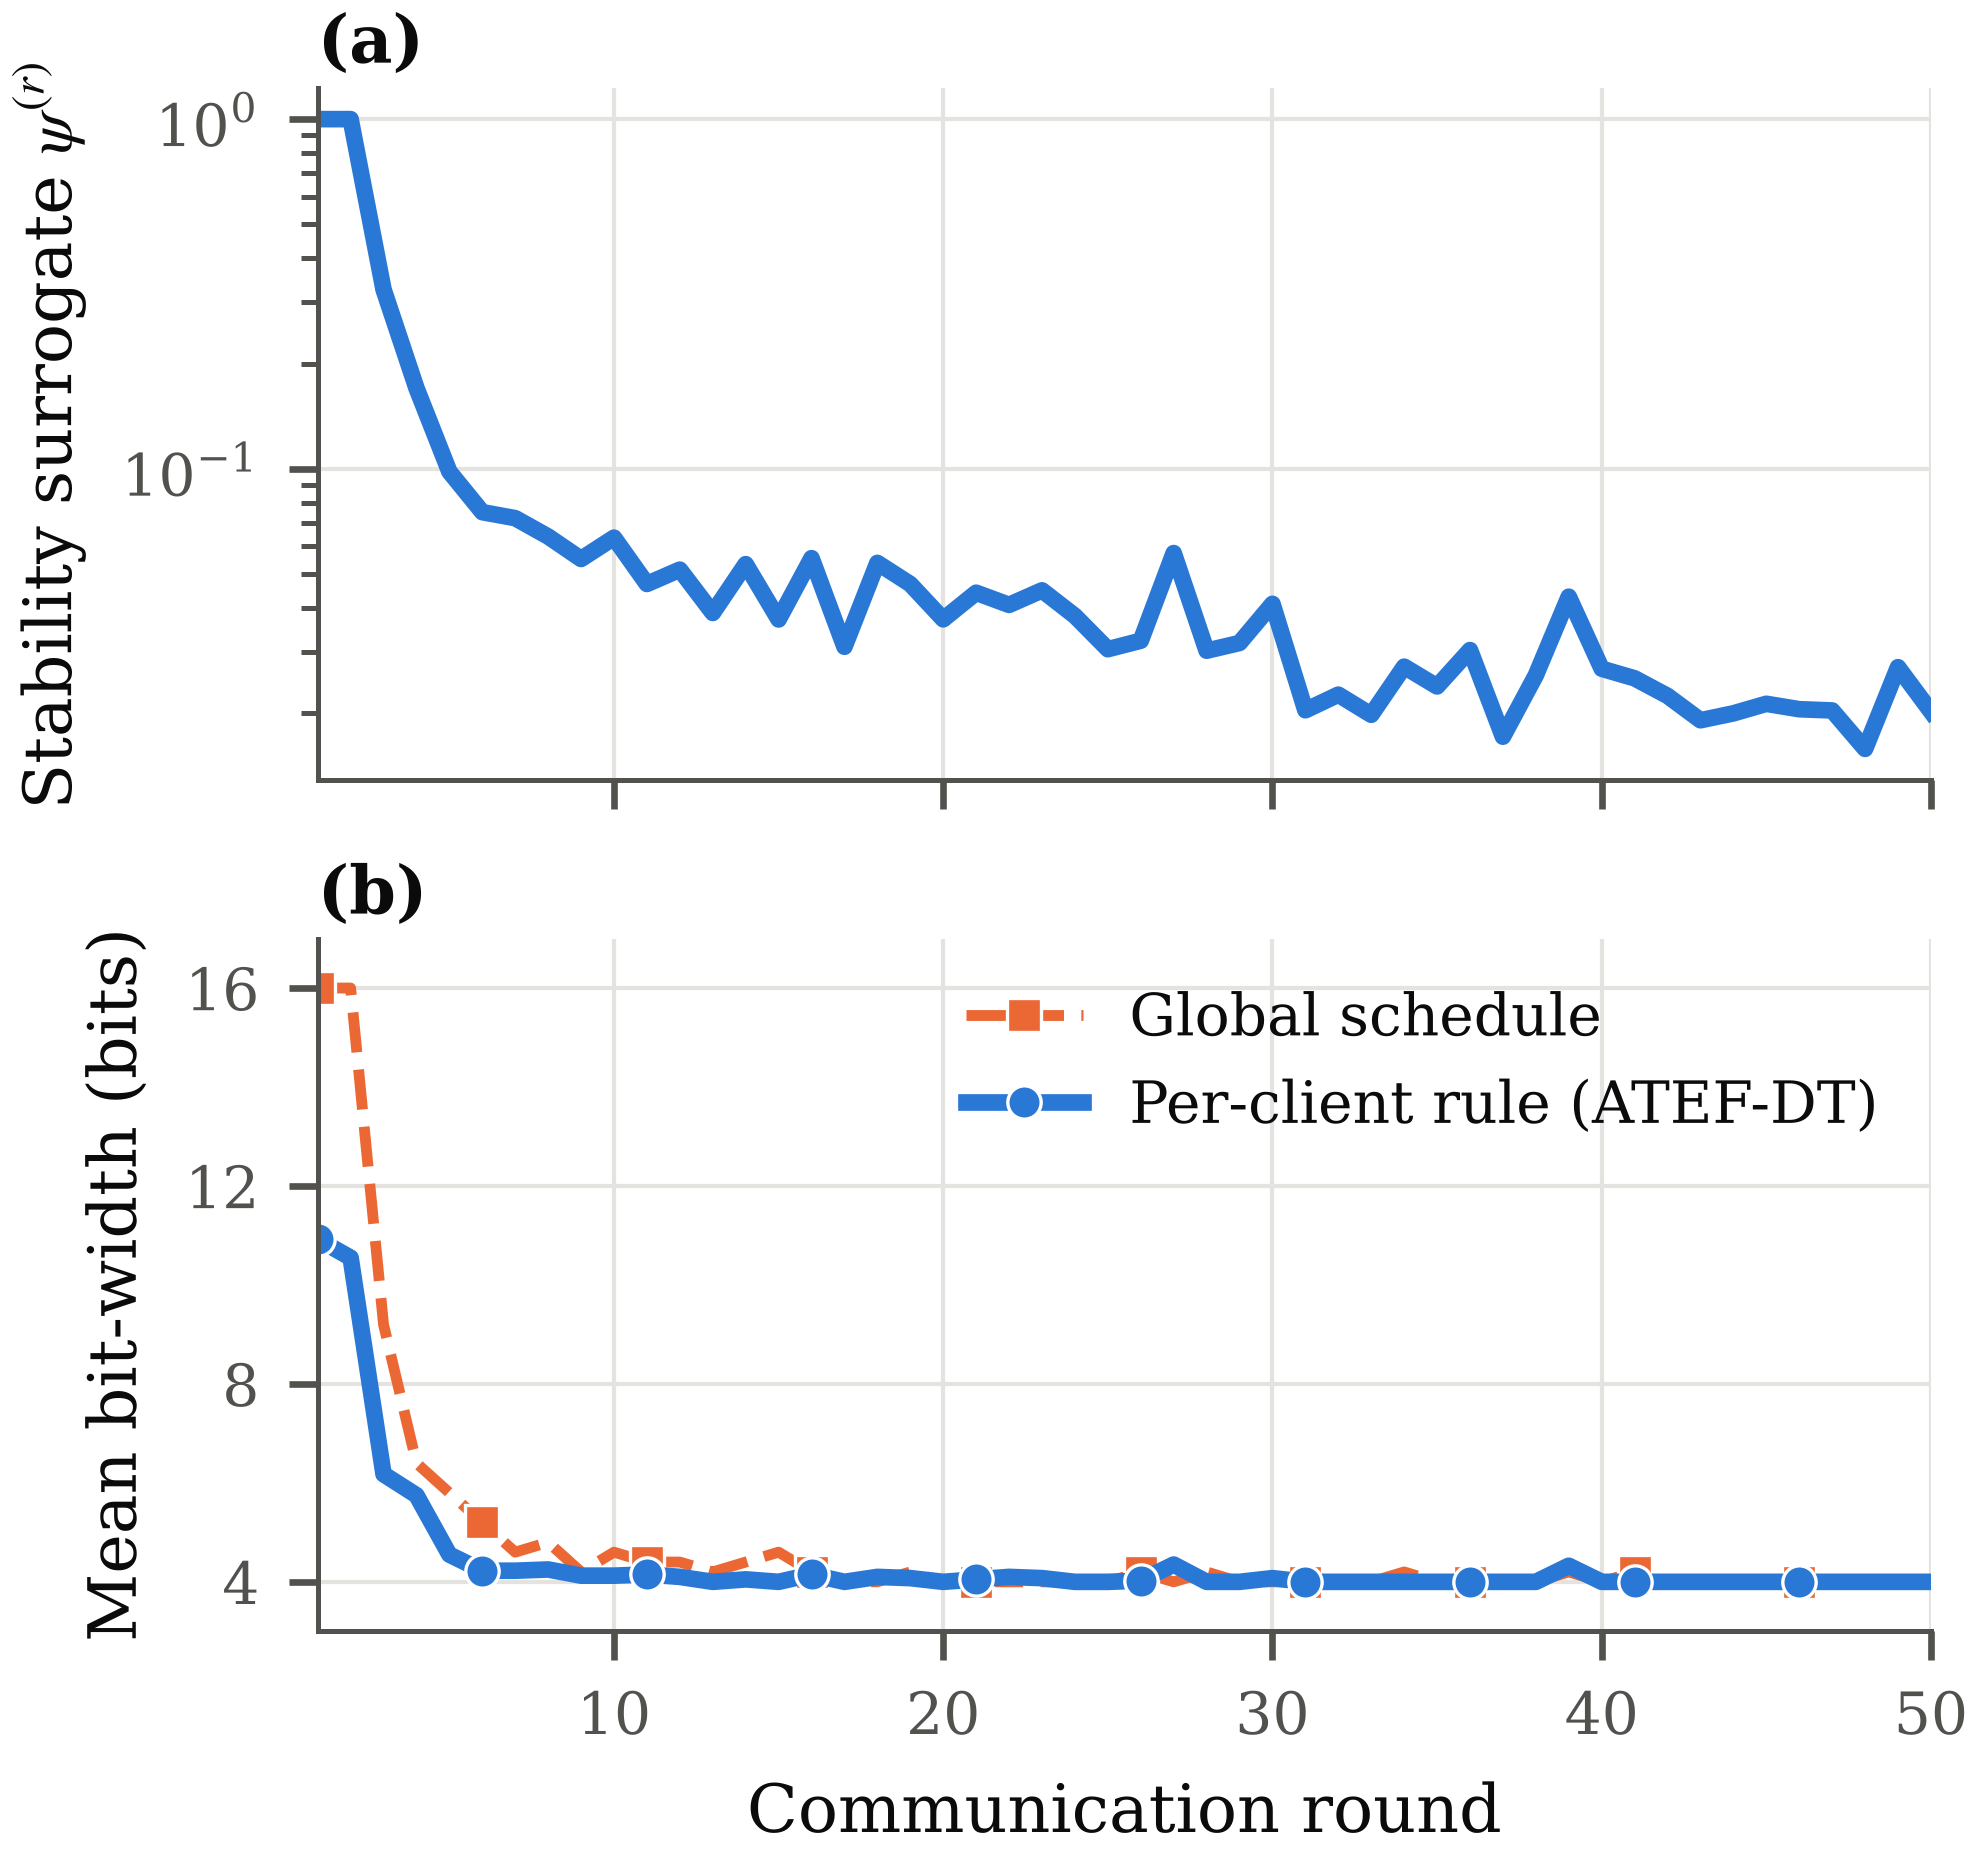
\includegraphics[width=\columnwidth]{figures/fig_bitwidth}
	\revcap{R1.7(1), R1.7(6)}{Adaptive quantization: (a)~stability surrogate $\psi^{(r)}$ and (b)~mean bit-width of the selected clients.}
	\label{fig:bitwidth}
\end{figure}

Computation dominates the account (\V{compshare-full}\% of the energy of FedAvg-Full), which is a consequence of the coefficient $\alpha$ of Table~\ref{tab:setup}. Section~\ref{subsec:sensitivity} varies $\alpha$ over three orders of magnitude; the default is the least favourable of the tested values for ATEF-DT.\end{revblock}

\rtag{R1.5}\begin{revblock}Table~\ref{tab:volume} compares four bit-width policies under the selection rule of ATEF-DT with full-precision transmission of the same updates. The per-client rule uses \V{meanb} bits per coordinate on average and reduces the uplink from \V{upMb-eftrust}~Mb to \V{upMb-atef2}~Mb, a factor of \V{compr}, in agreement with~\eqref{eq:compression}; the accuracy is unchanged within the variation across seeds. Figure~\ref{fig:bitwidth} shows why the mean is close to $b_{\min}$: the surrogate $\psi^{(r)}$ falls below $0.1$ within five rounds, after which nearly all transmissions use four bits. The reduction applies to the uplink only. The broadcast of the global model amounts to \V{downMb-atef}~Mb and the state reports to \V{stateMb}~Mb in every policy, so the total traffic falls from \V{totMb-eftrust}~Mb to \V{totMb-atef}~Mb, a reduction of \V{tot-red}\% and not of the \V{up-red}\% that the uplink alone would suggest.\end{revblock}

\subsection{Participation Fairness}
\label{subsec:fairres}
Figure~\ref{fig:fairness} shows the Jain index over the rounds. ATEF-DT reaches \Vpm{jain-atef}{jainsd-atef}, EA-FL \V{jain-eafl} and Energy+Trust \V{jain-etrust}; the latter two share the energy-greedy selection rule and return to the same clients. \rtag{R2.4}\rev{FedAvg-Random reaches \Vpm{jain-rand}{jainsd-rand}, in agreement with the expectation \V{jainexp} of~\eqref{eq:jainexp}; the small deficit is due to outages, which remove clients from some draws. The curve of FedAvg-Random in Figure~\ref{fig:fairness} follows the analytic curve throughout.} FedAvg-Full is below one (\V{jain-full}) for the same reason. FairFedCS reaches \V{jain-ffcs}: its queue grows in proportion to the reputation of a client, so it equalizes a reputation-weighted notion of fairness and not the raw participation counts that the Jain index measures.

\begin{figure}[t]
	\centering
	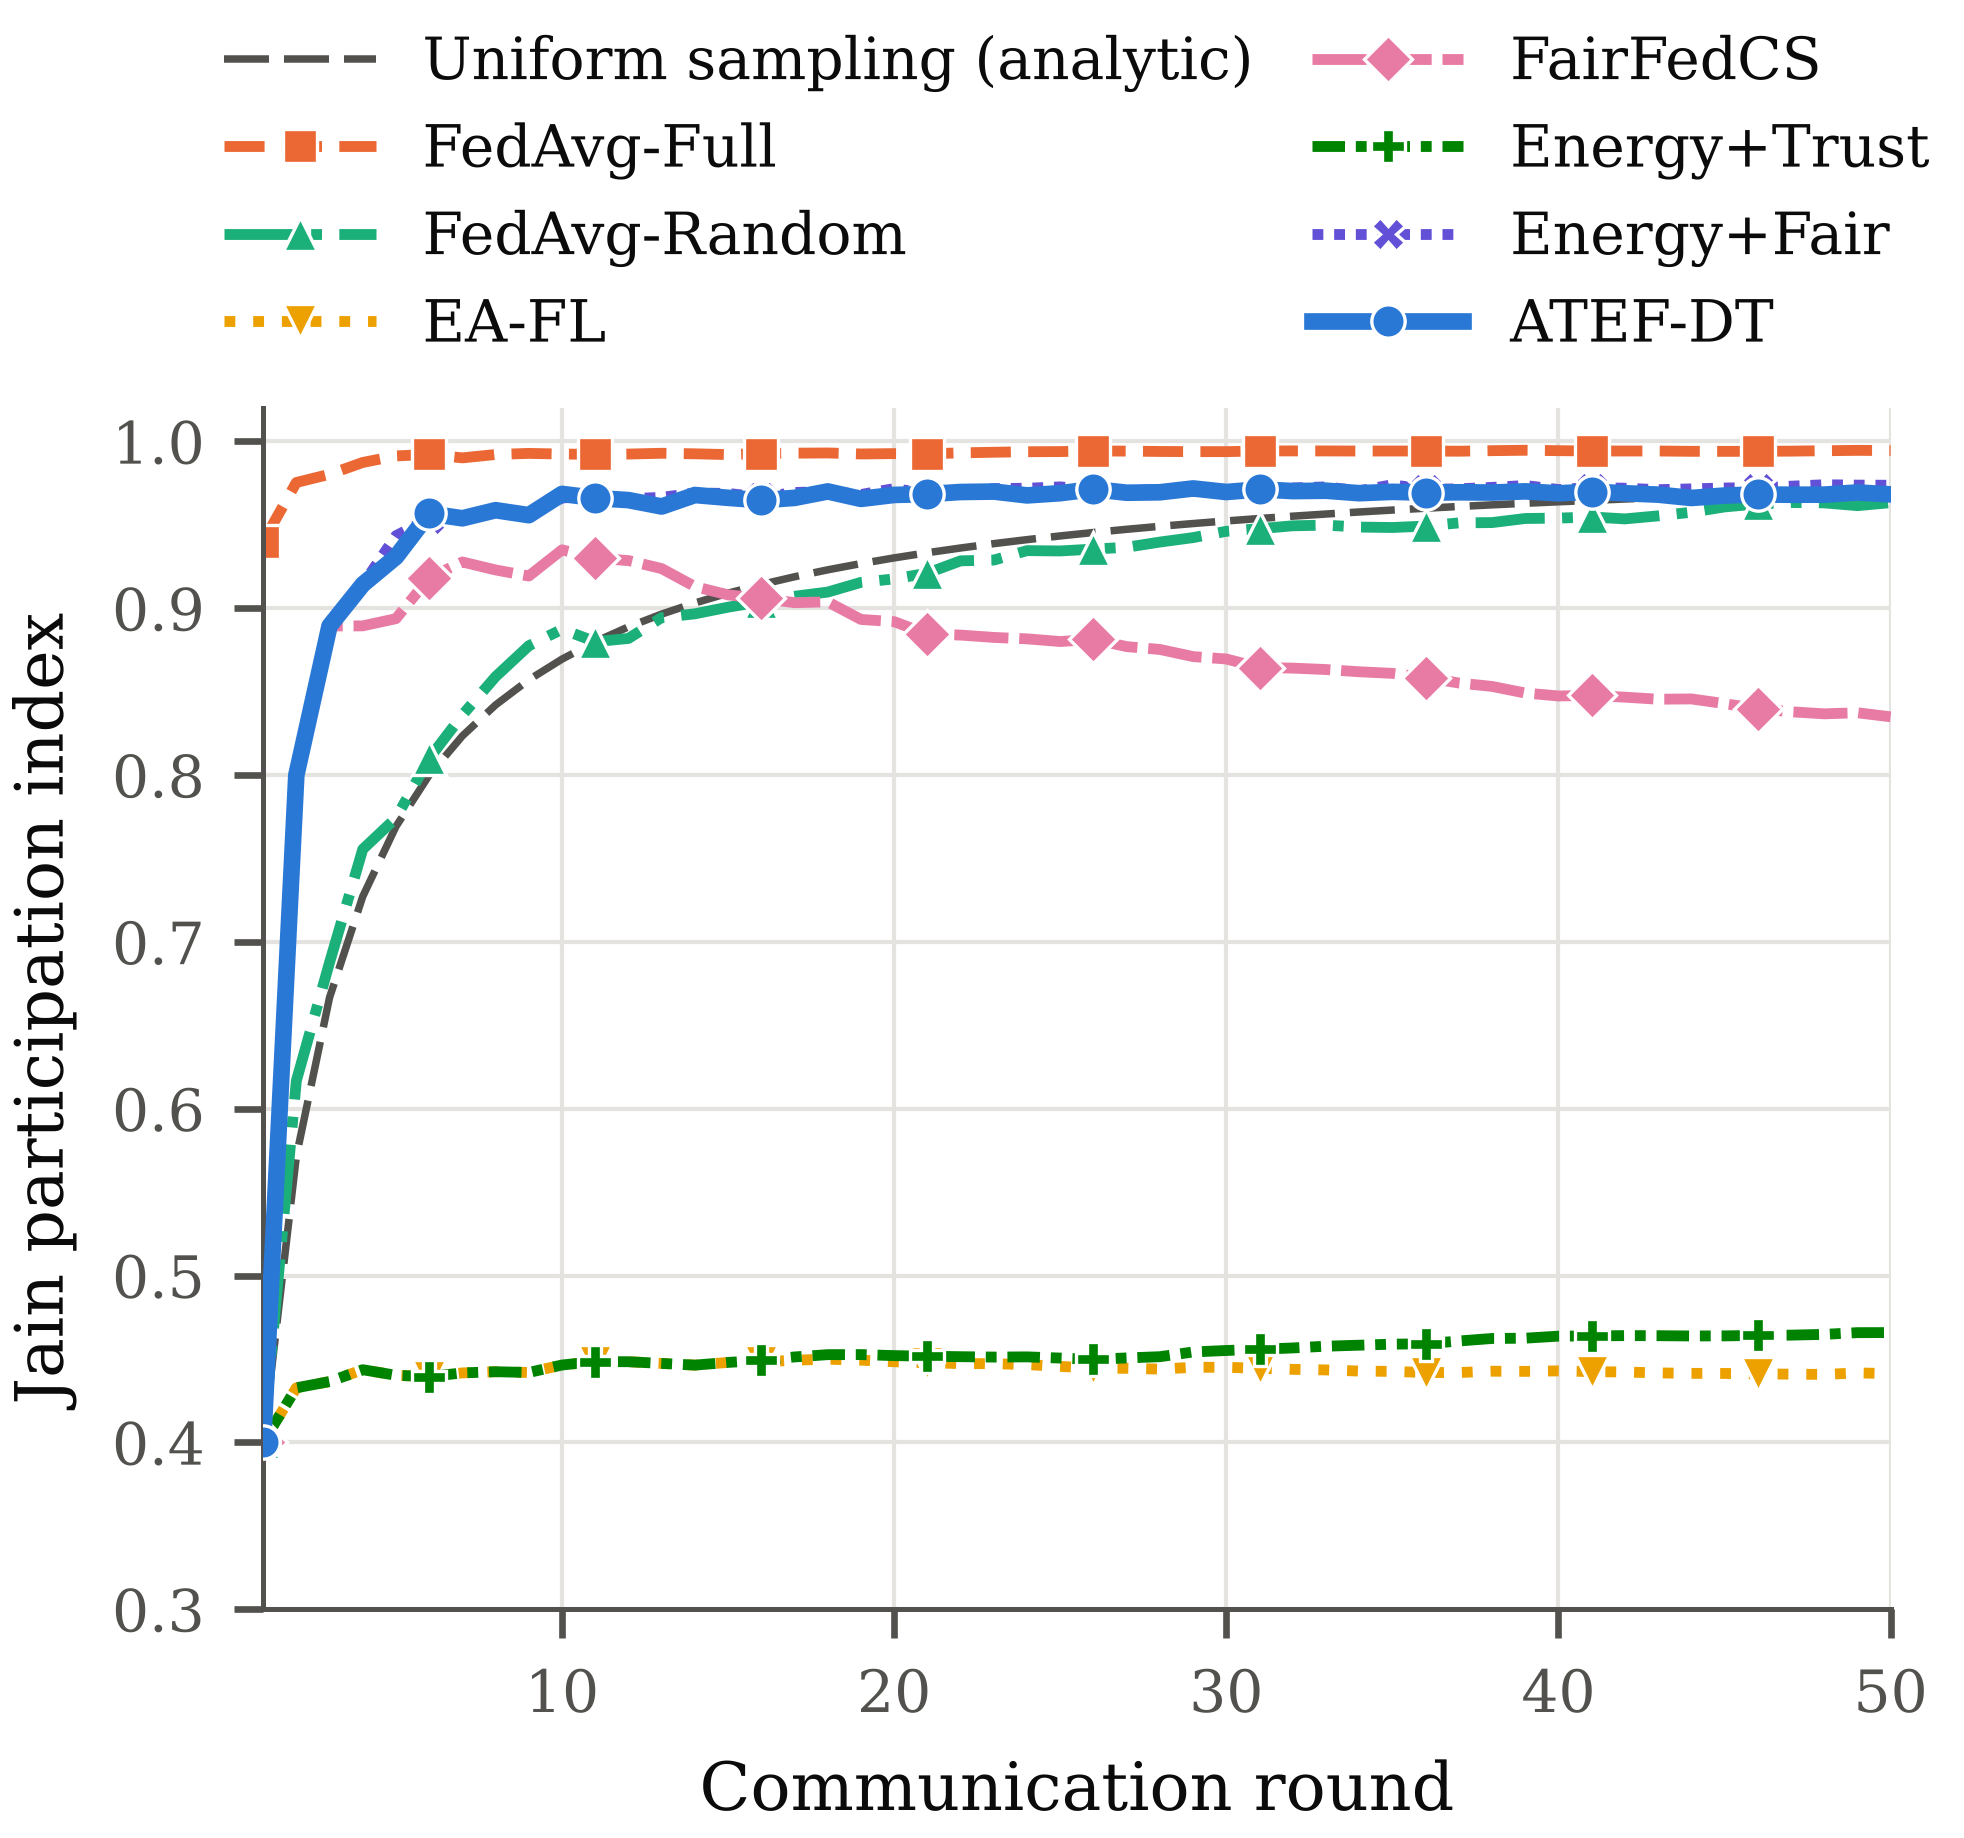
\includegraphics[width=\columnwidth]{figures/fig_fairness}
	\revcap{E4, R2.4}{Jain participation index; the dashed line is the expectation~\eqref{eq:jainexp} for uniform sampling.}
	\label{fig:fairness}
\end{figure}

\begin{table}[t]
	\centering
	\revcap{R1.5, E3}{Selection share and accuracy by device-resource tier, and distance of the effective weights from the data proportions.}
	\label{tab:group}
	\footnotesize
	\setlength{\tabcolsep}{2.5pt}
	\begin{tabular*}{\linewidth}{@{\extracolsep{\fill}}lccccc}
		\toprule
		 & \textbf{Share} & \multicolumn{2}{c}{\textbf{Accuracy (\%)}} & \textbf{Gap} & \\
		\cmidrule(lr){3-4}
		\textbf{Method} & \textbf{(\%)} & \textbf{High cost} & \textbf{Low cost} & \textbf{(pp)} & $\norm{\hat{\boldsymbol{\pi}}-\mathbf{n}/N}_1$ \\
		\midrule
		\tabin{tab_group}
		\bottomrule
	\end{tabular*}
\end{table}

\begin{figure*}[t]
	\centering
	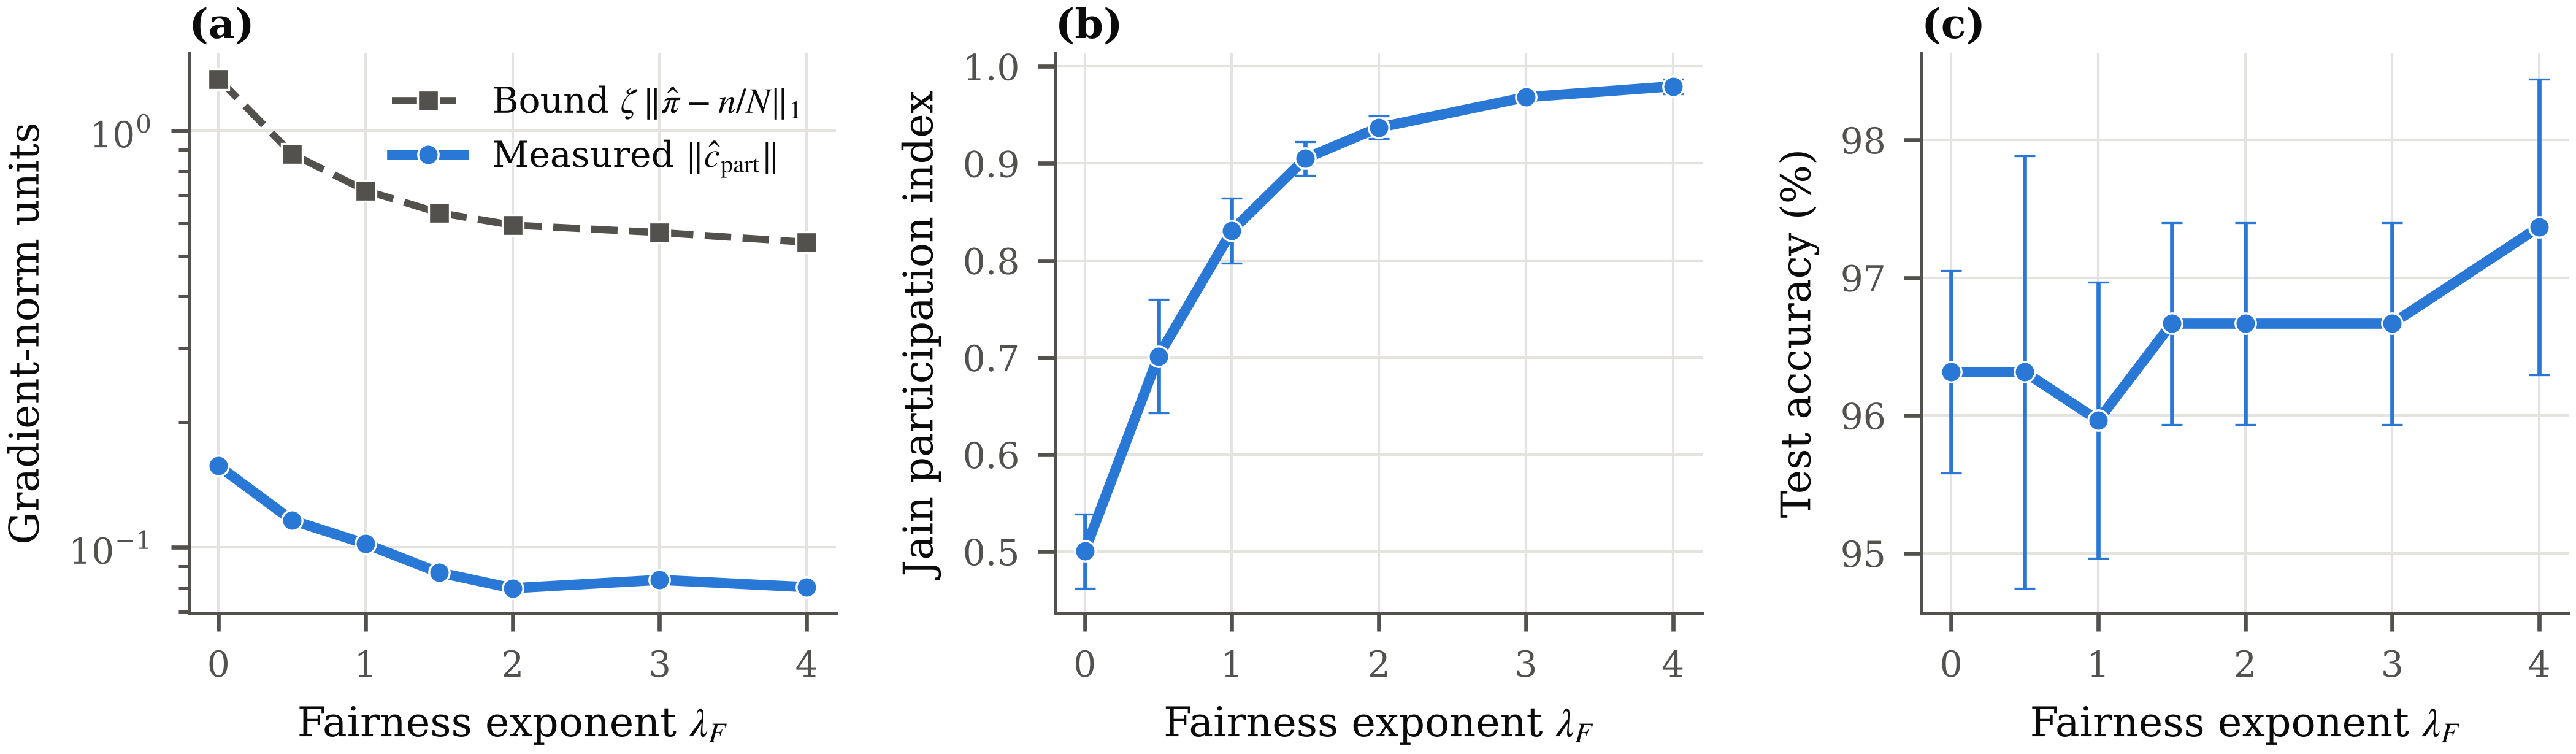
\includegraphics[width=\textwidth]{figures/fig_bias}
	\revcap{E3, R1.3, R2.3}{Effect of the fairness exponent $\lambda_F$: (a)~participation bias and its bound, (b)~Jain index and (c)~test accuracy.}
	\label{fig:bias}
\end{figure*}

\rtag{R1.5}\begin{revblock}The Jain index measures access to training. Whether unequal access harms the patients of the excluded devices is a separate question. To examine it, the clients are divided into two tiers by their static cost (computation energy plus full-precision uplink energy at the mean channel gain): a high-cost tier above the median and a low-cost tier below it. The test cases are assigned to clients with the class proportions of their training data, and accuracy is computed separately on the test cases of each tier. Table~\ref{tab:group} shows that EA-FL gives the high-cost tier \V{selhigh-eafl}\% of the selections and ATEF-DT \V{selhigh-atef}\%. The accuracy on the two tiers, however, differs by a few points at most for every method, with standard deviations of the same size, and EA-FL is not less accurate on the tier it excludes. On this data set, unequal participation does not translate into a consistent accuracy disparity between the tiers. The reason is that the features of WDBC are distributed similarly across clients, so a model trained on some clients serves the others. The fairness established here is therefore fairness of participation. WDBC contains no demographic or socio-economic attributes, and no claim is made about equity of outcomes for patient groups.\end{revblock}

\rtag{E3, R1.3, R2.3}\begin{revblock}Figure~\ref{fig:bias} varies $\lambda_F$ with the other exponents fixed. The Jain index rises from \V{jain-lf00} at $\lambda_F=0$ to \V{jain-lf40} at $\lambda_F=4$, and the energy from \V{E-lf00}~J to \V{E-lf40}~J. The accuracy stays between \V{acc-lf10}\% and \V{acc-lf40}\% without a trend that exceeds the variation across seeds. Panel~(a) reports the empirical counterpart of Proposition~\ref{prop:bias}: the effective weights are estimated by the run average $\hat{\boldsymbol{\pi}}=\sum_r\boldsymbol{\beta}^{(r)}/\sum_r s^{(r)}$, and the norm of $\sum_p(\hat\pi_p-N_p/N)\nabla f_p(\w^{(r)})$ and the bound $\zeta\norm{\hat{\boldsymbol{\pi}}-\mathbf{n}/N}_1$, with $\zeta$ the largest observed $\norm{\nabla f_p-\nabla F}$, are evaluated every ten rounds. The measured bias falls from \V{cpart-lf00} at $\lambda_F=0$ to \V{cpart-lf20} at $\lambda_F=2$ and is \V{cpart-lf30} at $\lambda_F=3$ and \V{cpart-lf40} at $\lambda_F=4$; it is not monotone, as anticipated in Section~\ref{subsec:bias}. The bound holds everywhere and is loose, by a factor of six to nine.

The last column of Table~\ref{tab:group} shows what the reputation weights cost. The distance of the effective weights from the data proportions is \V{pil1-efair} for Energy+Fair, which uses the same selection with data-volume weights, and \V{pil1-atef} for ATEF-DT. Most of the participation bias of ATEF-DT thus comes from the weighting and not from the selection. The measured step scale $s^{(r)}$ of ATEF-DT has a mean of \V{smean} and a minimum of \V{smin} over all rounds and seeds, well above the bound $\rho_{\min}/2$, so the condition $s_{\min}>0$ of Theorem~\ref{thm:convergence} is met in these runs.\end{revblock}

\subsection{Comparison With Multi-Objective Schedulers}
\label{subsec:schedulers}
\rtag{E1, R1.1, R2.1}\begin{revblock}This subsection tests the selection rule in isolation. Each of the five rules of Section~\ref{subsec:methods} has one parameter that trades energy against fairness: $\lambda_F$ for the weighted product and the weighted sum, $V$ for drift-plus-penalty, and the shortlist size $\bar k$ for the two pipelines. Each parameter is swept over a grid, and Figure~\ref{fig:frontier} shows the resulting energy--fairness curves, with FairFedCS, FedAvg-Random and EA-FL as single points. To compare the rules at equal fairness, a requirement of a Jain index of at least \V{jain-req} is imposed, and Table~\ref{tab:sched} reports, for each rule, the configuration on its grid that meets the requirement with the least energy.

\begin{figure}[t]
	\centering
	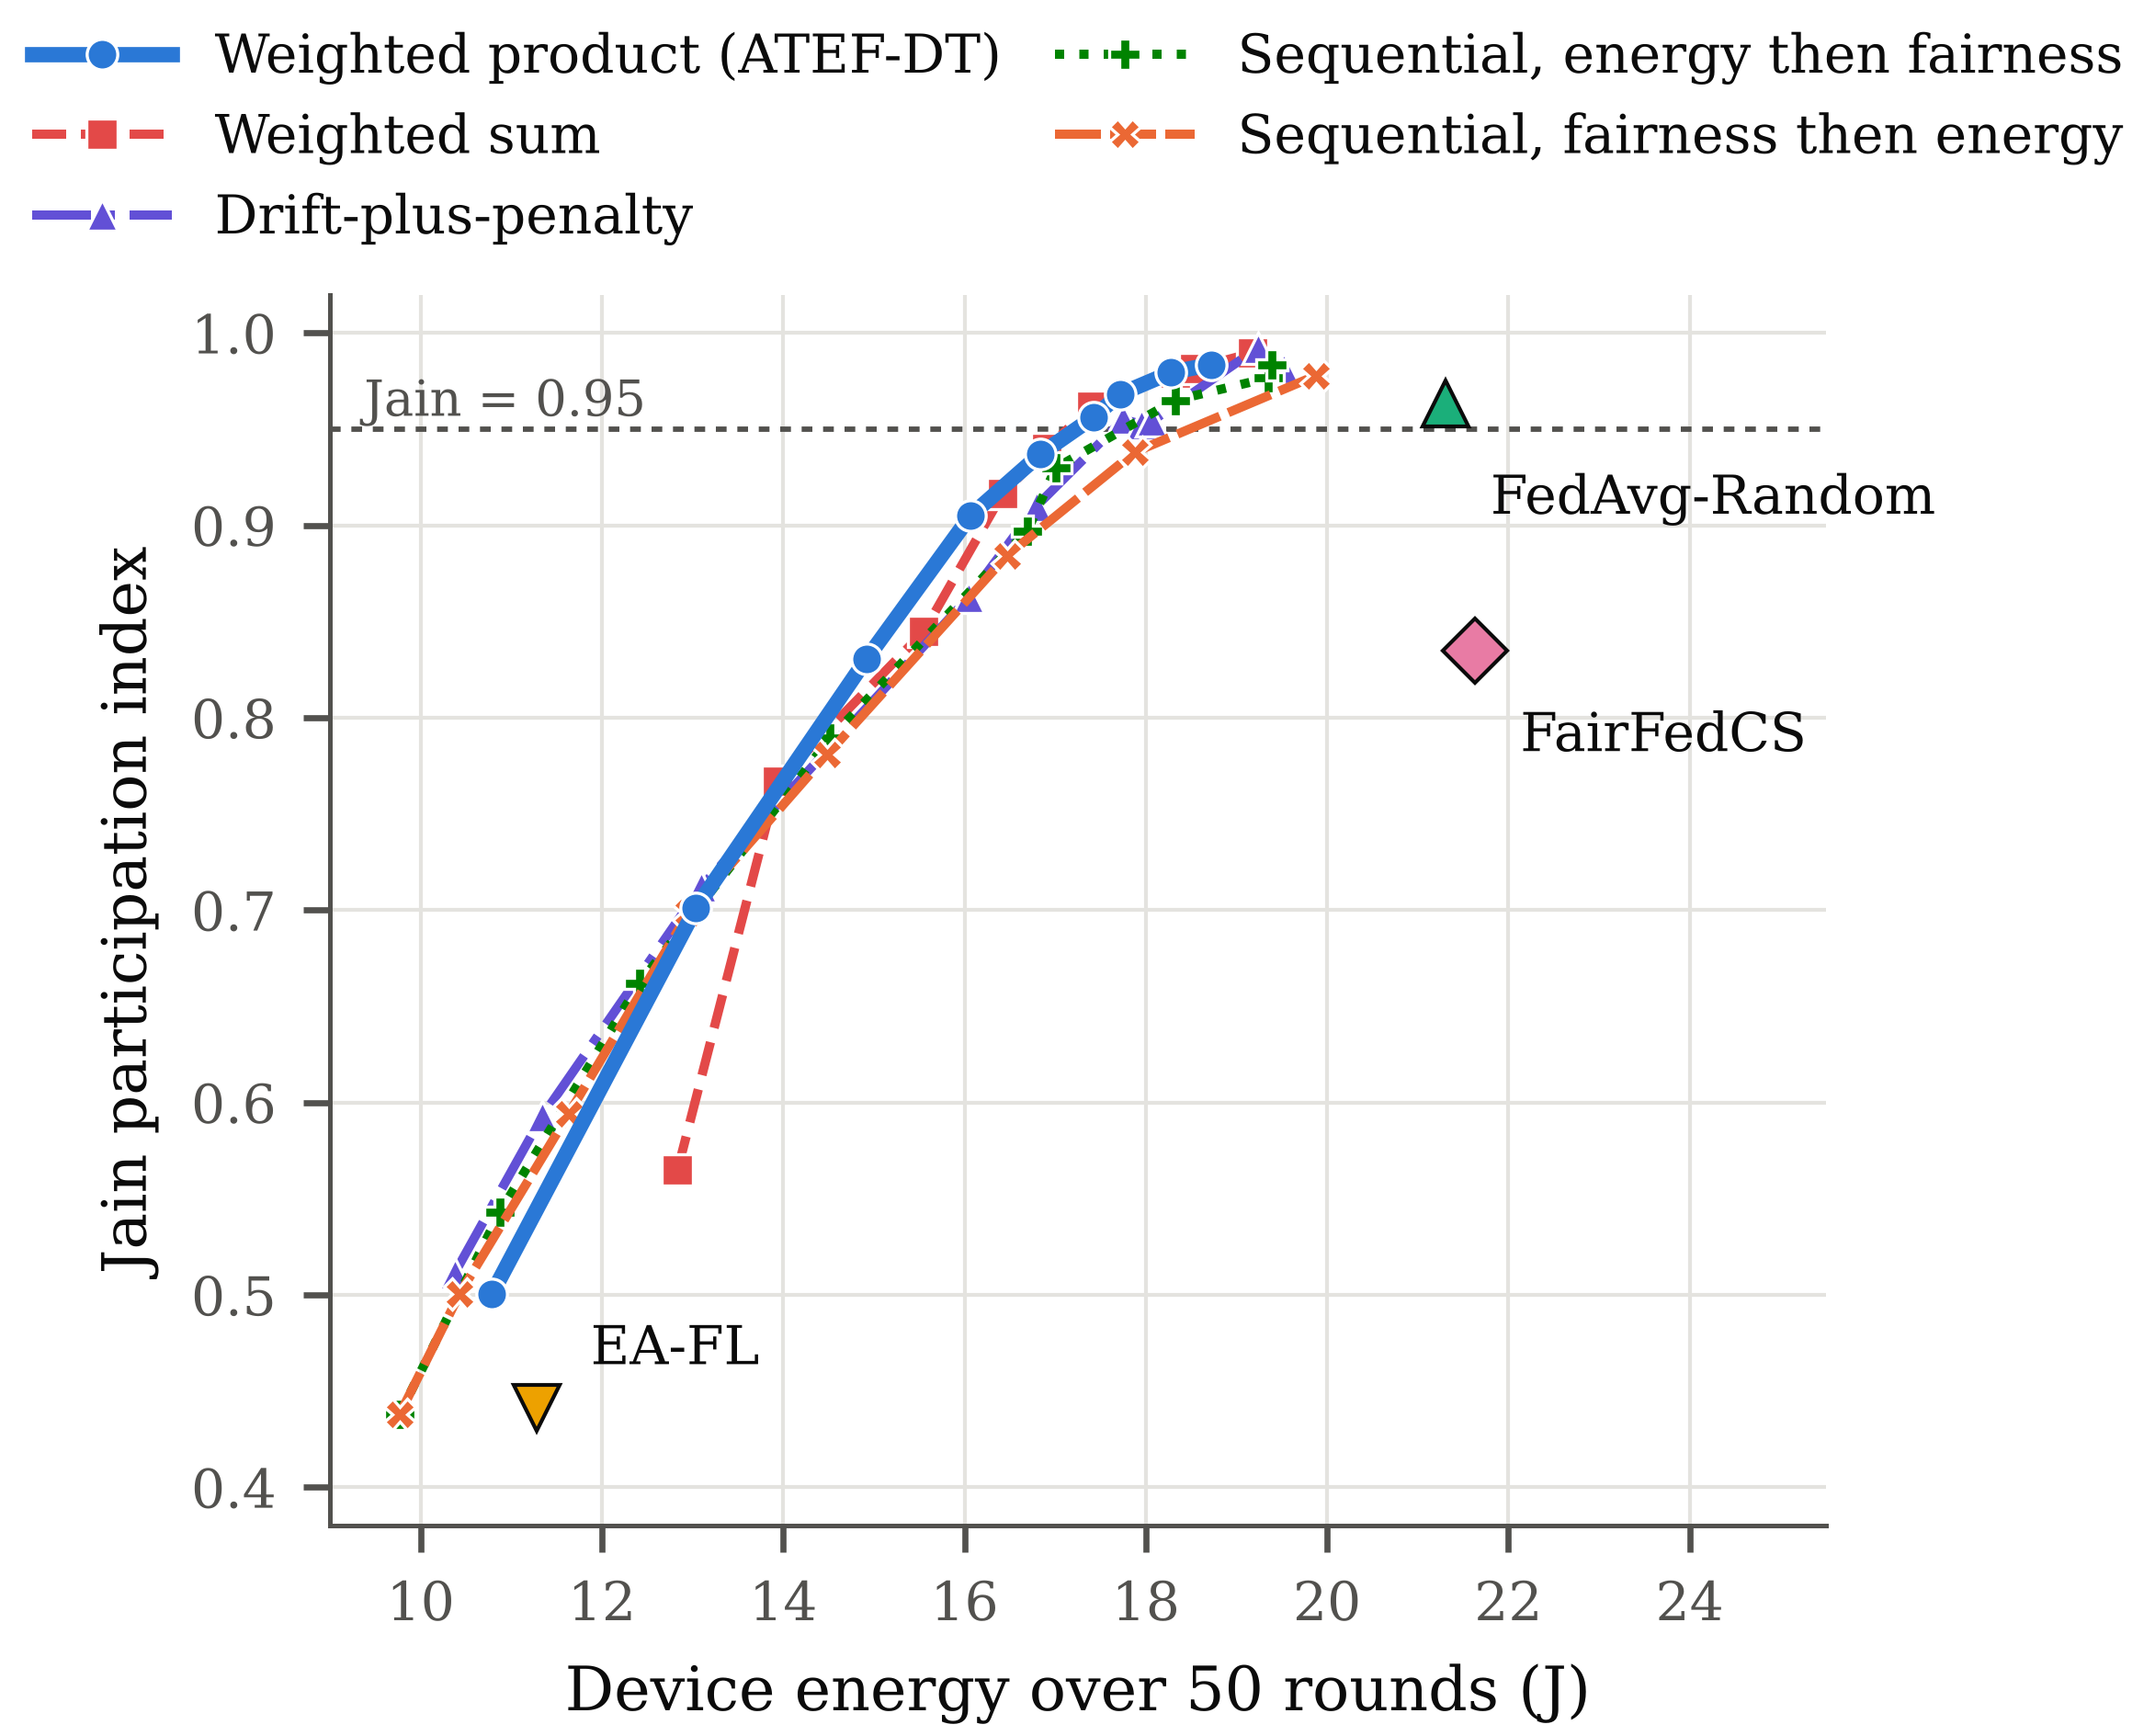
\includegraphics[width=\columnwidth]{figures/fig_frontier}
	\revcap{E1, R1.1, R2.1}{Energy--fairness curves of five selection rules.}
	\label{fig:frontier}
\end{figure}

\begin{table*}[t]
	\centering
	\revcap{E1, R1.1, R2.1}{Selection rules at a required Jain index of at least \V{jain-req}; the last column is the change in selections when the energy factor is scaled by $0.1$ / $10$.}
	\label{tab:sched}
	\footnotesize
	\begin{tabular*}{\linewidth}{@{\extracolsep{\fill}}llcccc}
		\toprule
		\textbf{Selection rule} & \textbf{Parameter} & \textbf{Jain index} & \textbf{Energy (J)} & \textbf{Accuracy (\%)} & \textbf{Change under rescaling (\%)} \\
		\midrule
		\tabin{tab_sched}
		\bottomrule
	\end{tabular*}
\end{table*}

Three findings follow. First, the three single-stage rules are indistinguishable. The weighted product needs \V{sched-E-prod}~J, the weighted sum \V{sched-E-add}~J and drift-plus-penalty \V{sched-E-dpp}~J; the paired differences to the weighted product are $\V{sched-diff-add}$~J ($p=\V{sched-p-add}$) and $\V{sched-diff-dpp}$~J ($p=\V{sched-p-dpp}$). At equal fairness, the weighted product is therefore as energy-efficient as a carefully tuned weighted sum. Second, the pipelines cost more. Seq-FE needs $\V{sched-diff-seqfe}$~J more than the weighted product ($p=\V{sched-p-seqfe}$); Seq-EF needs $\V{sched-diff-seqef}$~J more on average, a difference that is not significant over \V{nseeds} seeds ($p=\V{sched-p-seqef}$). Third, FairFedCS reaches a Jain index of \V{jain-ffcs} at \V{E-ffcs}~J: its index contains no energy term and its fairness notion is reputation-weighted, so it does not target this requirement.

The property that separates the weighted product from the weighted sum is Proposition~\ref{prop:scale}, and the last column of Table~\ref{tab:sched} measures it. When the energy factor is multiplied by $0.1$ or by $10$, with the exponents left at their default values, the selections of the weighted product do not change. Those of the weighted sum change by \V{resc-add-01}\% and \V{resc-add-10}\% of all selections, and under the factor $10$ its Jain index moves from \V{rescjain-add-1} to \V{rescjain-add-10} and its energy from \V{rescE-add-1}~J to \V{rescE-add-10}~J. A weighted sum therefore has to be re-tuned whenever the scale of a criterion changes, for instance with the hardware or the units, while the weighted product does not. This robustness to scaling, rather than a better energy--fairness trade-off, is the practical advantage of the product form.\end{revblock}

\subsection{Byzantine Robustness}
\label{subsec:byzantine}
Six attacks are simulated at adversarial fractions of 10\% to 40\% of the clients. \emph{Sign flipping} multiplies the update by $-1$; \emph{Gaussian poisoning} replaces it by a draw from $\mathcal{N}(\mathbf{0},(3\sigma_u)^2\mathbf{I})$, with $\sigma_u$ the root mean square of the honest update; \emph{label flipping} inverts the local labels before training; the \emph{scaled} attack multiplies the update by $10$; the \emph{backdoor} poisons half of the local samples with a trigger of four standard deviations on three features, targets the benign class and multiplies the update by $5$; and the \emph{adaptive} attack submits identical colluding updates at cosine $0.1$ to the mean honest update, along a common random direction and with the median honest norm. The adversaries are placed at random, independently for each seed, and attack from round~\V{attackstart}.

\begin{table}[t]
	\centering
	\caption{Test accuracy (\%) with 20\% adversarial clients.}
	\label{tab:byz}
	\footnotesize
	\begin{tabular*}{\linewidth}{@{\extracolsep{\fill}}lccc}
		\toprule
		\textbf{Method} & \textbf{No attack} & \textbf{Sign flipping} & \textbf{Label flipping} \\
		\midrule
		\tabin{tab_byz}
		\bottomrule
	\end{tabular*}
\end{table}

\begin{table*}[t]
	\centering
	\caption{Behaviour of the reputation layer of ATEF-DT under each attack with 20\% adversarial clients.}
	\label{tab:detail}
	\footnotesize
	\begin{tabular*}{\linewidth}{@{\extracolsep{\fill}}lccccccc}
		\toprule
		 & \textbf{Accuracy} & \textbf{Selection} & \textbf{Coefficient} & \textbf{Rejected} & \textbf{Adversaries} & \textbf{Honest} & \textbf{Success} \\
		\textbf{Attack} & \textbf{(\%)} & \textbf{share (\%)} & \textbf{share (\%)} & \textbf{(\%)} & \textbf{barred} & \textbf{barred (\%)} & \textbf{rate (\%)} \\
		\midrule
		\tabin{tab_detail}
		\bottomrule
	\end{tabular*}
\end{table*}

\begin{figure*}[t]
	\centering
	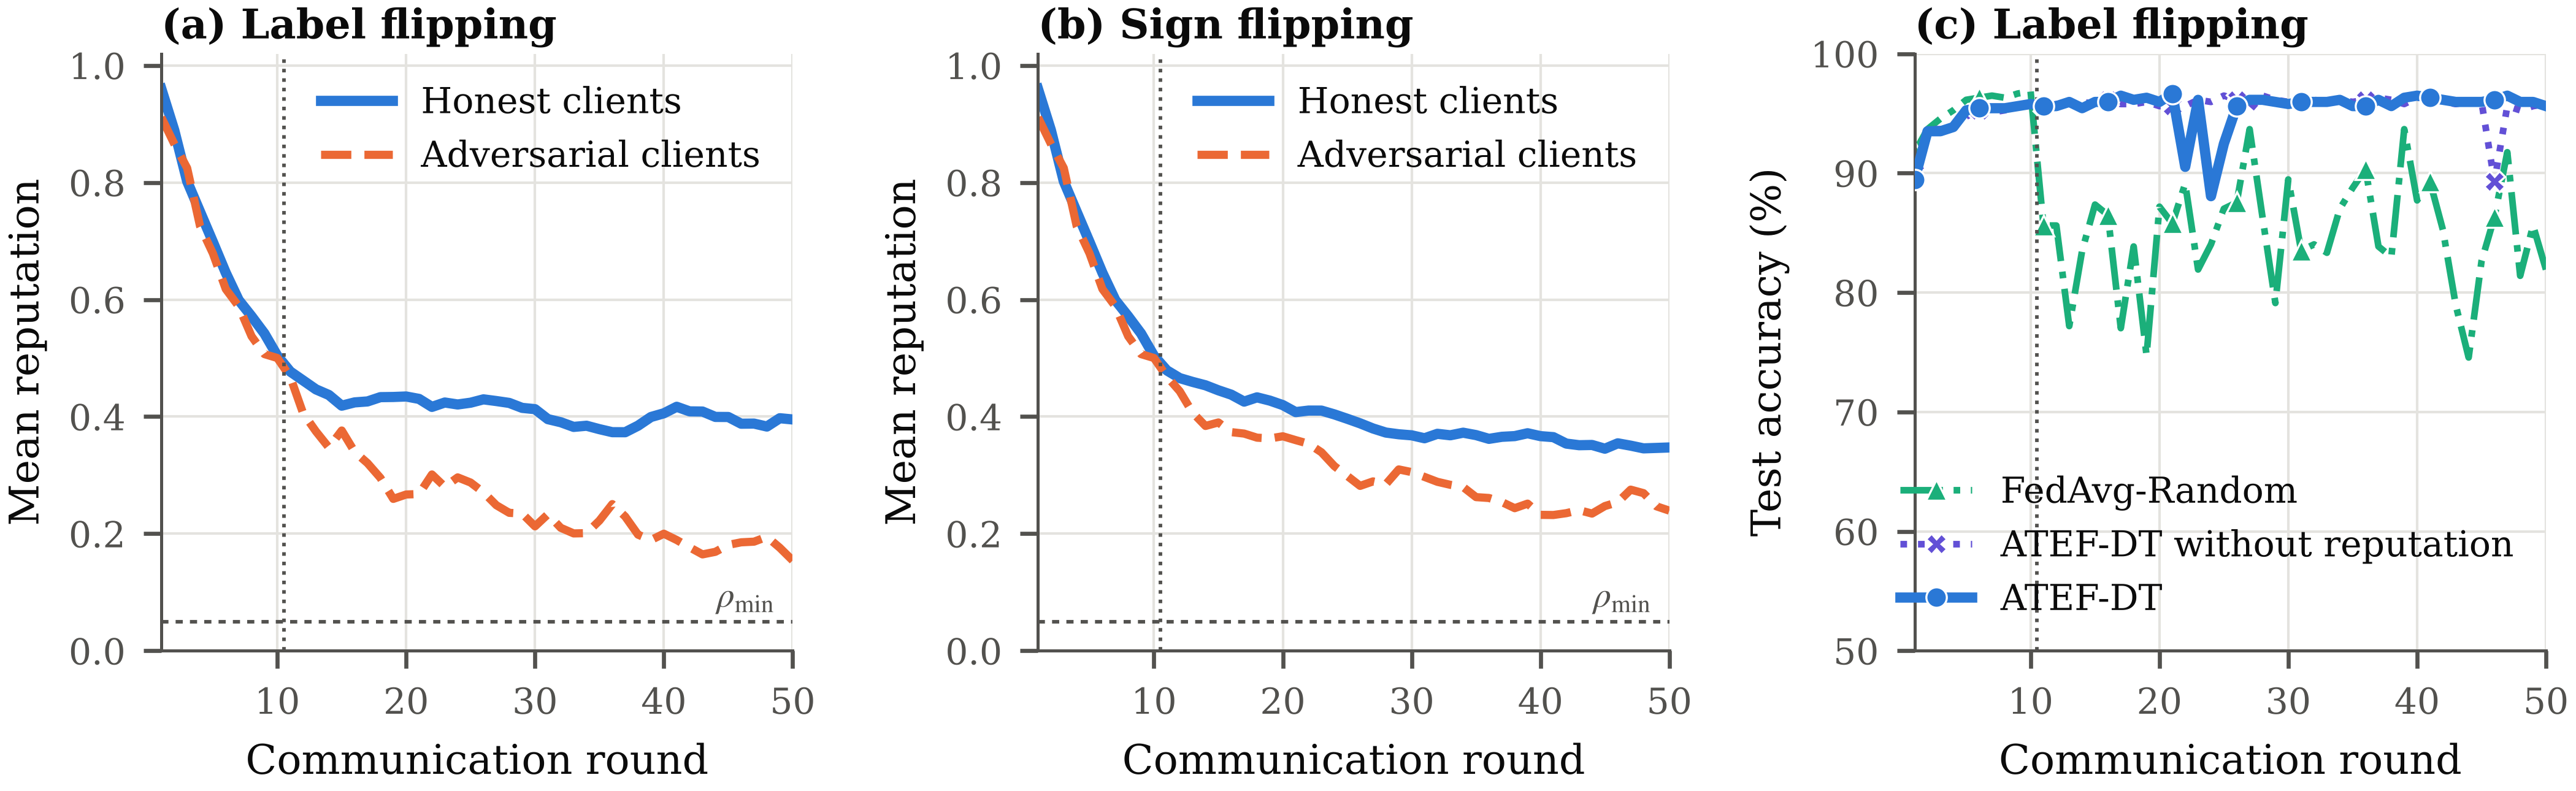
\includegraphics[width=\textwidth]{figures/fig_reputation}
	\revcap{R1.7(6)}{Reputations under (a)~label flipping and (b)~sign flipping, and (c)~accuracy under label flipping, with 20\% adversaries from round~\V{attackstart}.}
	\label{fig:reputation}
\end{figure*}

\begin{table*}[t]
	\centering
	\caption{Robust aggregation rules and matched variants.}
	\label{tab:robust}
	\footnotesize
	\begin{tabular*}{\linewidth}{@{\extracolsep{\fill}}lllccccc}
		\toprule
		 & & & \multicolumn{3}{c}{\textbf{Accuracy (\%)}} & \textbf{Energy} & \textbf{Jain} \\
		\cmidrule(lr){4-6}
		\textbf{Method} & \textbf{Selection} & \textbf{Aggregation} & \textbf{No attack} & \textbf{Sign flip} & \textbf{Label flip} & \textbf{(J)} & \textbf{index} \\
		\midrule
		\tabin{tab_robust}
		\bottomrule
	\end{tabular*}
\end{table*}

\begin{table}[t]
	\centering
	\caption{Test accuracy (\%) of ATEF-DT by attack and adversarial fraction.}
	\label{tab:grid}
	\footnotesize
	\setlength{\tabcolsep}{2.5pt}
	\begin{tabular*}{\linewidth}{@{\extracolsep{\fill}}lcccc}
		\toprule
		\textbf{Attack} & \textbf{10\%} & \textbf{20\%} & \textbf{30\%} & \textbf{40\%} \\
		\midrule
		\tabin{tab_grid}
		\bottomrule
	\end{tabular*}
\end{table}

\begin{table}[t]
	\centering
	\caption{Realized adversarial share of the selected set and rounds violating Assumption~\ref{ass:threat}.}
	\label{tab:realized}
	\footnotesize
	\begin{tabular*}{\linewidth}{@{\extracolsep{\fill}}ccc}
		\toprule
		\textbf{Adversarial} & \textbf{Mean share of the} & \textbf{Rounds violating} \\
		\textbf{clients (\%)} & \textbf{selected set (\%)} & \textbf{Assumption~\ref{ass:threat} (\%)} \\
		\midrule
		\tabin{tab_realized}
		\bottomrule
	\end{tabular*}
\end{table}

\begin{table}[t]
	\centering
	\caption{Test accuracy (\%) with 30\% and 40\% adversarial clients.}
	\label{tab:high}
	\footnotesize
	\setlength{\tabcolsep}{2pt}
	\begin{tabularx}{\columnwidth}{>{\raggedright\arraybackslash}X cccc}
		\toprule
		 & \multicolumn{2}{c}{\textbf{Sign flipping}} & \multicolumn{2}{c}{\textbf{Label flipping}} \\
		\cmidrule(lr){2-3}\cmidrule(lr){4-5}
		\textbf{Method} & \textbf{30\%} & \textbf{40\%} & \textbf{30\%} & \textbf{40\%} \\
		\midrule
		\tabin{tab_high}
		\bottomrule
	\end{tabularx}
\end{table}

\begin{table*}[t]
	\centering
	\caption{Sensitivity of the reputation layer to $\mu$ and $\rho_{\min}$ (default marked with an asterisk).}
	\label{tab:trustsens}
	\footnotesize
	\begin{tabular*}{\linewidth}{@{\extracolsep{\fill}}cccccccc}
		\toprule
		 & & & \textbf{Honest barred,} & \textbf{Accuracy} & \textbf{Coefficient} & \textbf{Adversaries} & \textbf{Honest} \\
		$\boldsymbol{\mu}$ & $\boldsymbol{\rho_{\min}}$ & $\boldsymbol{k^{\star}}$ & \textbf{no attack (\%)} & \textbf{(\%)} & \textbf{share (\%)} & \textbf{barred} & \textbf{barred (\%)} \\
		\midrule
		\tabin{tab_trustsens}
		\bottomrule
	\end{tabular*}
\end{table*}

\begin{table*}[t]
	\centering
	\revcap{E4, R1.7(2)}{Functional test of the twin layer with synthetic streams and small batteries.}
	\label{tab:twin}
	\footnotesize
	\begin{tabular*}{\linewidth}{@{\extracolsep{\fill}}lccccc}
		\toprule
		\textbf{Feasibility screen} & \textbf{Reserve breaches} & \textbf{Client-rounds with} & \textbf{Transmissions} & \textbf{Jain index} & \textbf{Accuracy (\%)} \\
		 & \textbf{after participation} & \textbf{empty battery} & & & \\
		\midrule
		\tabin{tab_twin}
		\bottomrule
	\end{tabular*}
\end{table*}

Table~\ref{tab:byz} compares the methods under sign flipping and label flipping. Label flipping is the more damaging attack in this setting: FedAvg-Random falls to \Vpm{lf20-rand}{lf20sd-rand}\% and EA-FL to \V{lf20-eafl}\%, while ATEF-DT retains \Vpm{lf20-atef}{lf20sd-atef}\% (paired $p=\V{p-lf-atef-rand}$ against FedAvg-Random; the large spread of the baseline across seeds limits the power of the test). Under sign flipping the methods are closer (\V{sf20-rand}\% for FedAvg-Random, \V{sf20-atef}\% for ATEF-DT), because a flipped full-batch gradient of a minority only shortens the average step.

Table~\ref{tab:detail} reports the behaviour of the reputation layer for each attack at 20\%, and Figure~\ref{fig:reputation} shows the reputations over time. Under label flipping the adversaries receive \V{g-malsel-lf20}\% of the selections but carry only \V{g-malw-lf20}\% of the aggregation coefficients: their reputation falls and the weights~\eqref{eq:agg} follow. The gate plays a minor part. Only \V{g-bar-lf20} of \V{g-nadv-lf20} adversaries are barred within the run, and \V{g-rej-lf20}\% of the received malicious updates are rejected. The exclusion time $k^{\star}=\V{kstar}$ of Lemma~\ref{lem:rep} is rarely attained, because its premise, a trust signal that is never positive, does not hold: each received update is itself part of the set from which the reference is computed, which gives every update a positive alignment with the reference, of the order of $1/\sqrt{k}$ for $k$ otherwise uncorrelated updates of comparable norm, and as training approaches a stationary point the honest updates lose their common direction, so the signal no longer separates the two populations. Figure~\ref{fig:reputation} shows this: the mean reputation of honest clients settles near $0.4$, not near one, and that of the adversaries declines slowly. The reputation layer thus acts through graded weights and not through exclusion. In clean runs it bars \V{fe-clean}\% of the honest clients, and such an exclusion is permanent.

Table~\ref{tab:robust} places ATEF-DT beside four robust aggregation rules and beside its own variants without the reputation layer. At 20\% adversaries the methods are close. The variant that keeps the clipping and replaces the reputation weights by an unweighted mean reaches \V{lf20-norep}\% under label flipping and \V{sf20-norep}\% under sign flipping, against \V{lf20-atef}\% and \V{sf20-atef}\% for ATEF-DT ($p=\V{p-lf-atef-norep}$ for label flipping), and the geometric median with uniform selection reaches \V{lf20-gm}\% and \V{sf20-gm}\%. At this adversarial fraction, clipping accounts for most of the robustness of ATEF-DT, and the reputation weights add no measurable accuracy. What ATEF-DT offers over the robust aggregation baselines is the same robustness at lower energy (\V{E-atef}~J against \V{E-rand}~J), since those baselines select uniformly at full precision.

Table~\ref{tab:grid} gives the accuracy of ATEF-DT for all attacks and fractions, and Table~\ref{tab:realized} the realized composition of the selected sets. Up to 20\% the accuracy stays within 1.3 points of the clean value for every attack. At 30\% it holds under label flipping (\V{g-acc-lf30}\%) and becomes unstable under sign flipping (\Vpm{g-acc-sf30}{g-accsd-sf30}\%). At 40\% the method fails under both (\V{g-acc-sf40}\% and \V{g-acc-lf40}\%). The failure has a definite cause: with 40\% adversarial clients, adversaries are at least half of the selected set in \V{viol-40}\% of the rounds, which violates Assumption~\ref{ass:threat}; in such rounds the reference is captured, the adversaries gain reputation and the honest clients lose it, and the reputations carry the error into later rounds. Table~\ref{tab:high} shows the consequence. Beyond the domain of Assumption~\ref{ass:threat} the memory of the reputation layer is a liability: under sign flipping at 40\%, ATEF-DT (\V{hi-sf40-dt}\%) is far below its own variant without reputation (\V{hi-sf40-norep}\%) and below the geometric median (\V{hi-sf40-gm}\%), whereas under label flipping at 30\% it is above both.

Against the backdoor the protection is partial. With 20\% adversaries the attack success rate is \V{g-asr-bd20}\% for ATEF-DT, against \V{asr20-rand}\% for FedAvg-Random; at 10\% it is \V{g-asr-bd10}\%. The variant without reputation (\V{asr20-norep}\%) and the geometric median (\V{asr20-gm}\%) do at least as well, so the reduction is due to clipping and the reputations do not contribute to it. The clean accuracy is hardly affected by the backdoor, which would therefore not be noticed from the accuracy. The adaptive adversary exposes the second part of Assumption~\ref{ass:threat}. Its colluders submit identical vectors at a small positive cosine to the honest mean. Identical vectors attract the geometric median, the colluders are then closer to the reference than the honest clients, and the engine rewards them: at 20\% they receive \V{g-malsel-ad20}\% of the selections and \V{g-malw-ad20}\% of the aggregation coefficients, and at 40\% they hold \V{g-malw-ad40}\% of the coefficients while \V{g-fe-ad40}\% of the honest clients are barred. The accuracy remains high in Table~\ref{tab:grid} only because the direction that this adversary injects is random and not chosen to increase the loss. Against colluding clients the credibility engine does not protect the model.

Table~\ref{tab:trustsens} varies the forgetting factor and the threshold. Raising the threshold to $0.10$ bars more adversaries and many honest clients; a longer memory ($\mu=0.8$) bars almost none of either. The share of the coefficients carried by label-flipping adversaries stays below three per cent in all configurations, and the accuracy is 95\% or higher in all but one. These observations confirm that the weights, and not the gate, carry the protection, and that the gate could be removed at little cost. When the attack starts at round~0 instead of round~\V{attackstart}, the accuracy under label flipping is \V{on0-lf-acc}\% and under sign flipping \V{on0-sf-acc}\%. A variant in which the reference~\eqref{eq:gm} is weighted by the reputations was examined and rejected: it couples the reference to its own output, and in clean runs it barred \V{wref-fe}\% of the honest clients and lowered the Jain index to \V{wref-jain}. It remains available as an option in the released code.

\rtag{E4, R1.5, R1.7(2)}\begin{revblock}WDBC has no physiological stream, and with the batteries of Table~\ref{tab:setup} the screen~\eqref{eq:screen} never binds. The twin layer is therefore tested on its own, with synthetic streams and small batteries; the learning task is unchanged. Each patient has $m=3$ standardized vital-sign deviations that follow a mean-reverting process, and half of the patients undergo a deterioration episode during the run, in which the mean rises over eight rounds to between $0.75$ and $4$ standard deviations depending on the variable. Measurements carry Gaussian noise of standard deviation $\V{twc-twinrsd}$ and are missing in 20\% of the rounds. The batteries are drawn uniformly from $[\V{twc-batterylow},\V{twc-batteryhigh}]$~J, with a reserve of \V{twc-Cres}~J and $C_{\mathrm{ref}}=\V{twc-Cref}$~J. The streams are generated by a model that differs from the twin model~\eqref{eq:twinmodel}, so that the twin is not tested on data from its own model class.

Table~\ref{tab:twin} compares three screens: the twin forecast~\eqref{eq:screen}, an instantaneous test $C_p^{(r)}-\hat e_p^{(r)}\ge C_{\mathrm{res}}$, and no reserve. The first column counts the participations that are followed, within $H$ rounds, by a fall of the battery below the reserve. The twin forecast reduces these events from \V{tw-breach-none} to \V{tw-breach-twin} per run, against \V{tw-breach-instant} for the instantaneous test, and it reduces the client-rounds with an empty battery. It does so by withdrawing devices earlier, which lowers the Jain index from \V{tw-jain-none} to \V{tw-jain-twin} and the accuracy from \V{tw-acc-none}\% to \V{tw-acc-twin}\%. The screen thus trades participation for monitoring continuity, as intended, and it does not remove the events entirely, because an episode that starts after a participation cannot be foreseen.

The tracking error shows what the filter contributes. The mean absolute error of the local-level twin is \V{tw-mae-level} standardized units, against \V{tw-mae-hold} when the last received measurement is held and \V{tw-mae-ar} for the autoregressive alternative. The advantage of filtering grows with the sensor noise: at a noise of $0.40$ the errors are \V{tw-mae-level-04} and \V{tw-mae-hold-04}, and at $0.10$ they are \V{tw-mae-level-01} and \V{tw-mae-hold-01}, so that with accurate sensors holding the last measurement is almost as good. The autoregressive model, fitted on a resting window, reverts to rest during an episode and is not better than holding at low noise (\V{tw-mae-ar-01}); this is the reason for adopting the local-level model. These results establish that the twin layer functions as specified on synthetic data. They do not establish its clinical validity.\end{revblock}

\subsection{Ablation}
\label{subsec:ablation}
Table~\ref{tab:ablation} and Figure~\ref{fig:ablation} add the components one at a time. The fairness factor (C1 to C2) raises the Jain index from \V{jain-eafl} to \V{jain-efair} and the energy from \V{E-eafl}~J to \V{E-efair}~J. The reputation layer (C2 to C3) leaves energy and fairness essentially unchanged, lowers the clean accuracy slightly, from \V{acc-efair}\% to \V{acc-eftrust}\%, and raises the accuracy under label flipping from \V{lf20-efair}\% to \V{lf20-eftrust}\%; as shown in Section~\ref{subsec:byzantine}, most of this gain is due to clipping. Adaptive quantization (C3 to C4) reduces the uplink from \V{upMb-eftrust}~Mb to \V{upMb-atef}~Mb and the energy to \V{E-atef}~J without loss of accuracy.

\begin{table*}[t]
	\centering
	\caption{Ablation of ATEF-DT; each row adds one component to the previous one.}
	\label{tab:ablation}
	\footnotesize
	\begin{tabular*}{\linewidth}{@{\extracolsep{\fill}}lccccc}
		\toprule
		\textbf{Configuration} & \textbf{Accuracy (\%)} & \textbf{Energy (J)} & \textbf{Jain index} & \textbf{Uplink (Mb)} & \textbf{Label flip (\%)} \\
		\midrule
		\tabin{tab_ablation}
		\bottomrule
	\end{tabular*}
\end{table*}

\begin{figure*}[t]
	\centering
	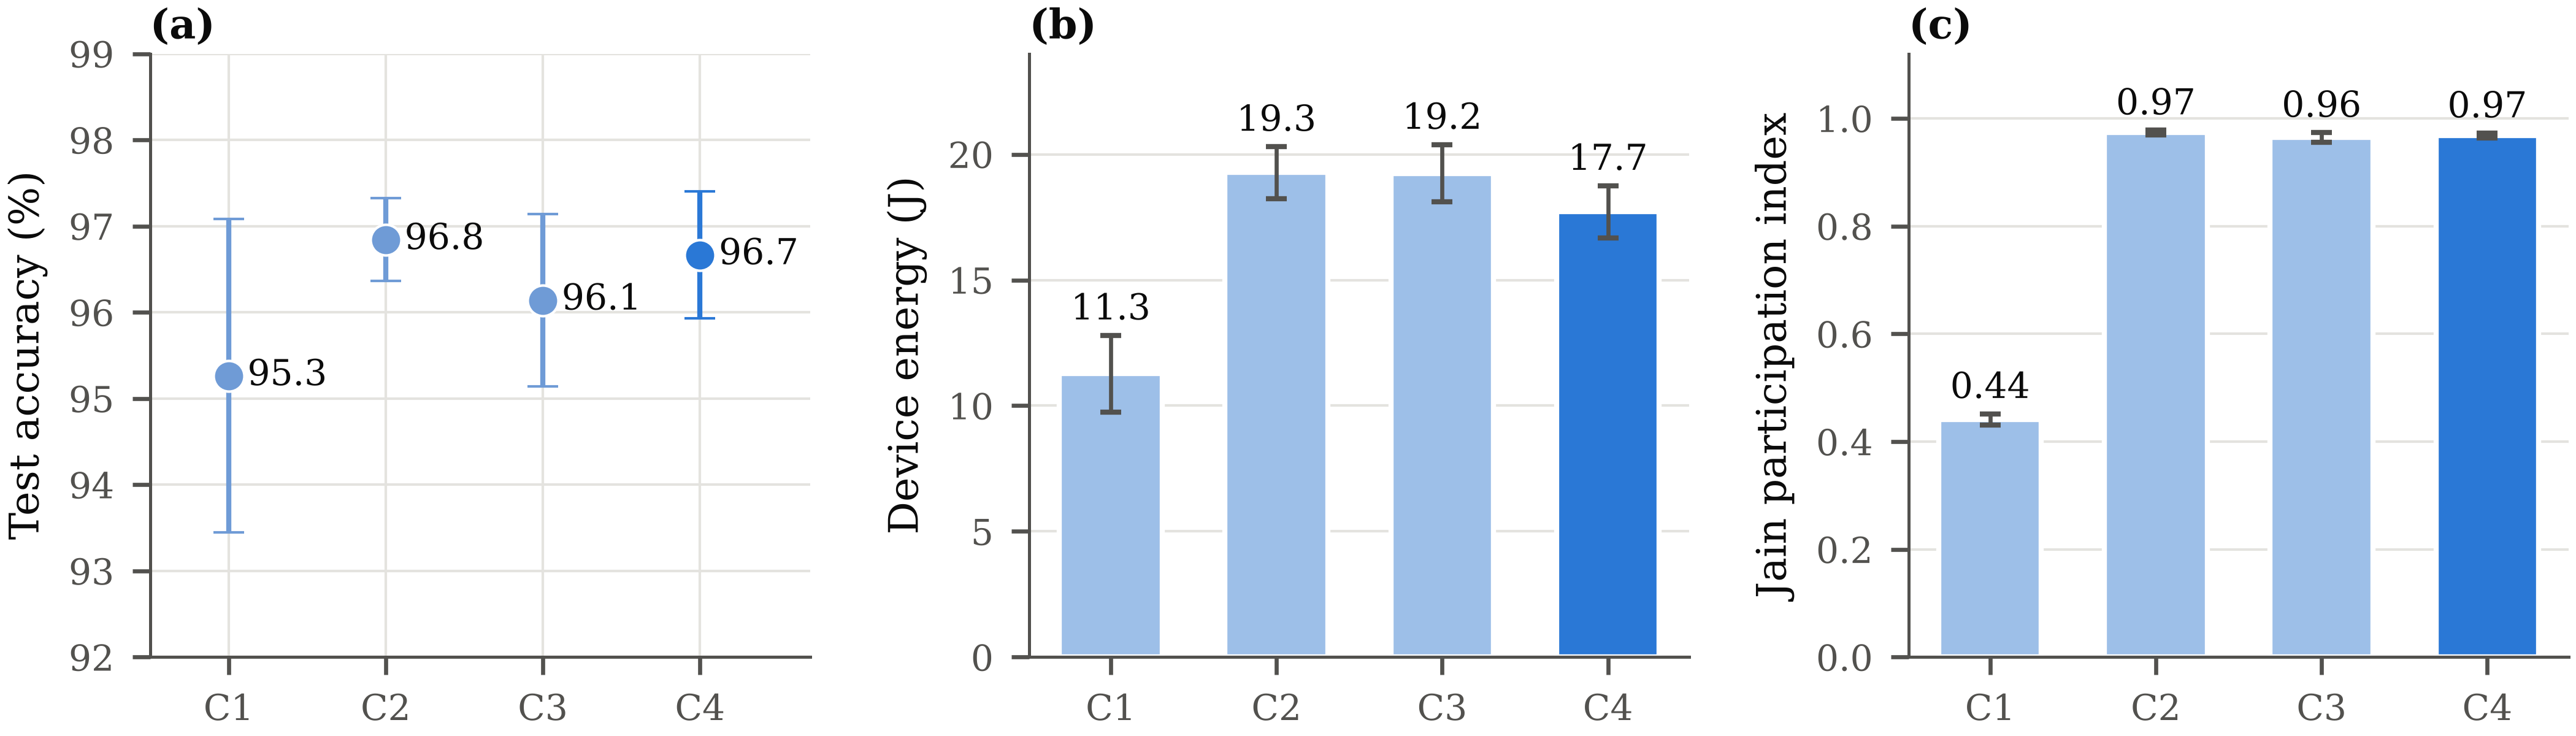
\includegraphics[width=\textwidth]{figures/fig_ablation}
	\revcap{R1.7(6)}{Ablation: (a)~test accuracy, (b)~device energy and (c)~Jain index.}
	\label{fig:ablation}
\end{figure*}

\subsection{Scalability and Overhead}
\label{subsec:scalability}
The population is increased from 20 to \V{pmax} clients with the budget kept at 40\% of the clients. Since WDBC is small, the clients of this experiment draw their data from the training set with replacement, with the same label skew; a larger population therefore does not mean more distinct data, and the experiment tests the scheduler and the server, not the statistical benefit of more clients. Figure~\ref{fig:scalability} shows that the Jain index of ATEF-DT stays between \V{sc-jain-atef-200} and \V{sc-jain-atef-20}, its energy per client near one joule, below that of FedAvg-Random at every size, and its accuracy between \V{sc-acc-atef-20}\% and \V{sc-acc-atef-200}\%.

\begin{figure*}[t]
	\centering
	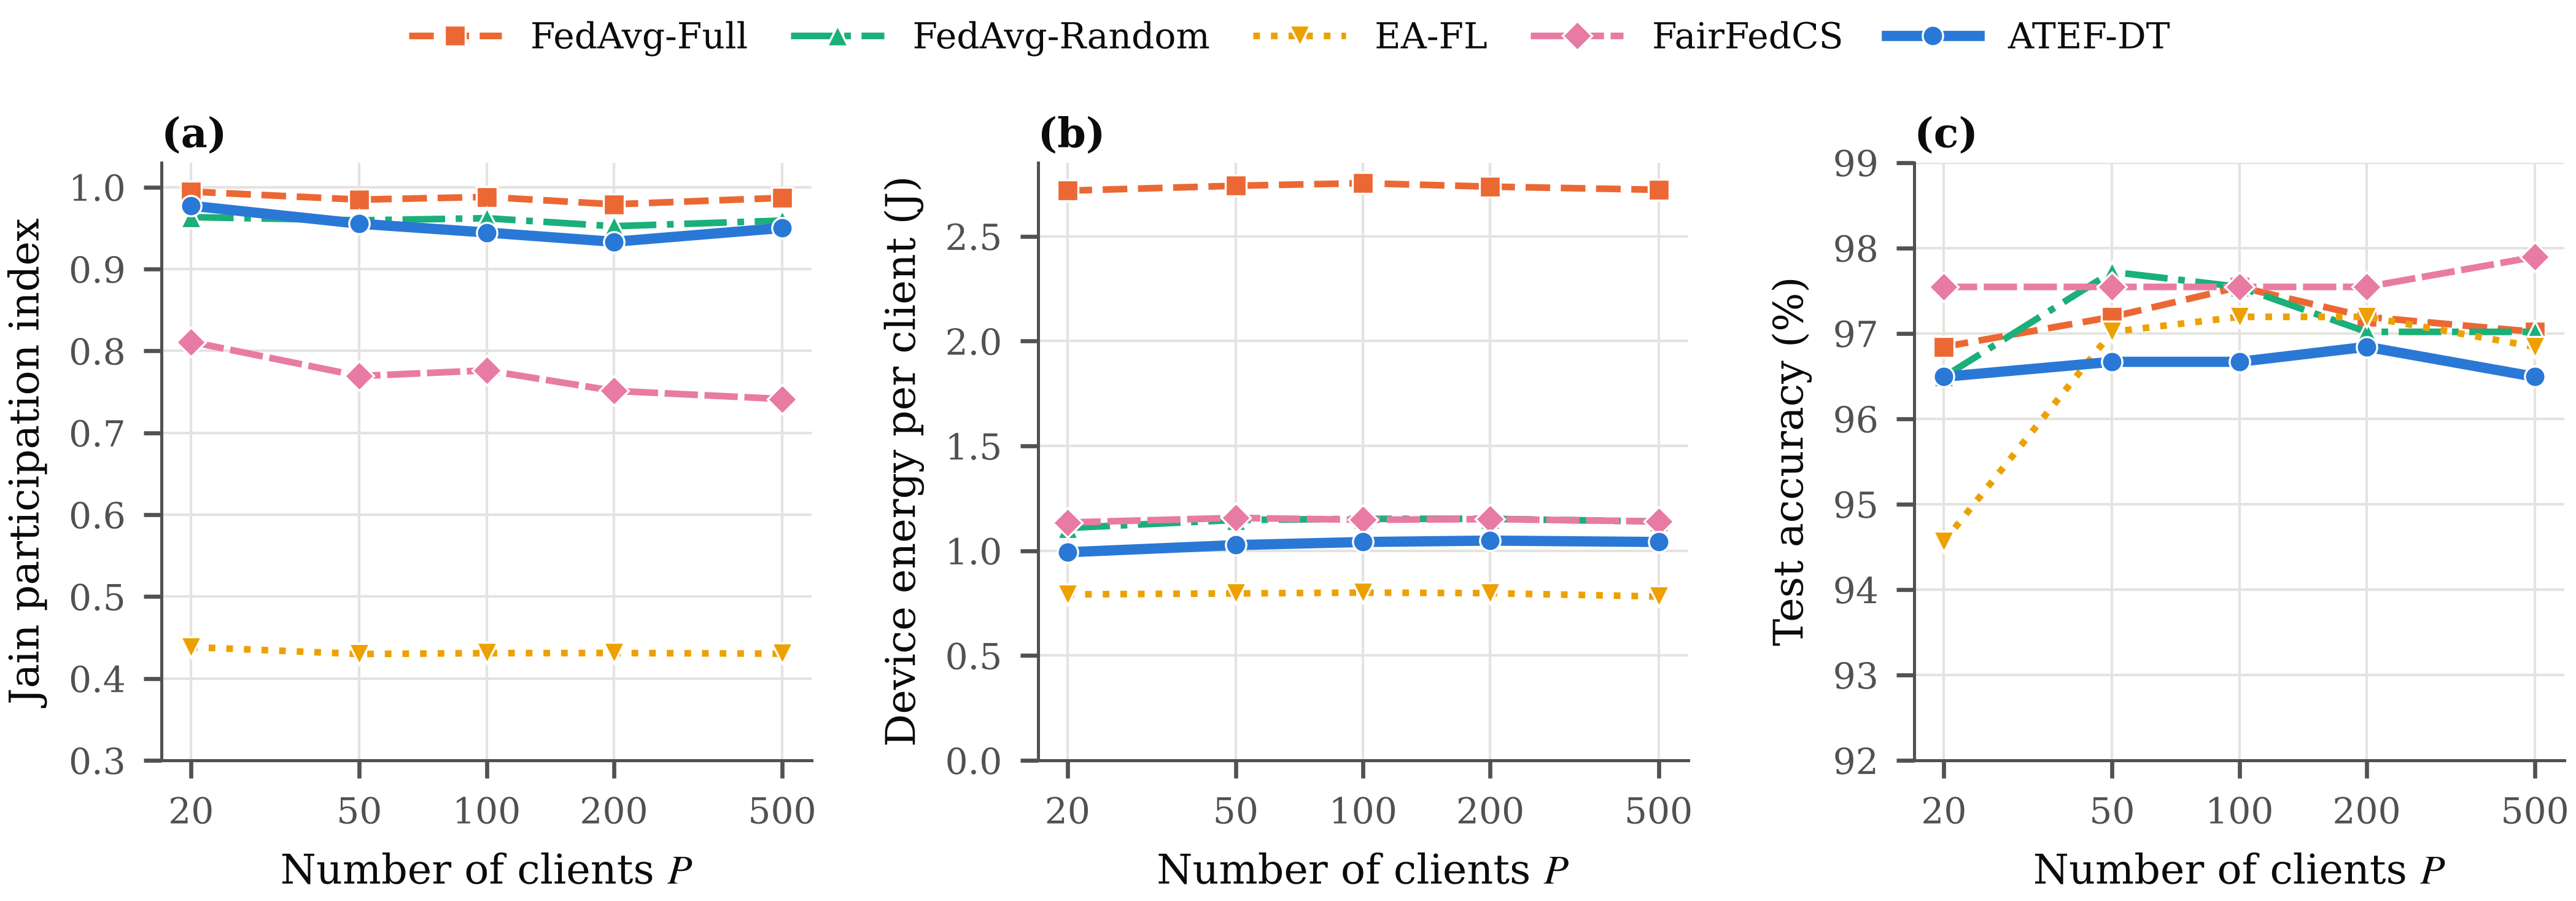
\includegraphics[width=\textwidth]{figures/fig_scalability}
	\revcap{R1.7(6)}{Scalability from 20 to \V{pmax} clients: (a)~Jain index, (b)~energy per client and (c)~test accuracy.}
	\label{fig:scalability}
\end{figure*}

\begin{table*}[t]
	\centering
	\revcap{E5}{Server-side time per round (ms).}
	\label{tab:overhead}
	\footnotesize
	\begin{tabular*}{\linewidth}{@{\extracolsep{\fill}}cccccccc}
		\toprule
		\textbf{Clients} & \textbf{Selected} & \textbf{Scoring and} & \textbf{Geometric} & \textbf{Weiszfeld} & \textbf{Reputation} & \textbf{Clipping and} & \textbf{Total} \\
		$\boldsymbol{P}$ & \textbf{per round} & \textbf{selection} & \textbf{median} & \textbf{iterations} & \textbf{update} & \textbf{aggregation} & \\
		\midrule
		\tabin{tab_overhead}
		\bottomrule
	\end{tabular*}
\end{table*}

\begin{figure*}[t]
	\centering
	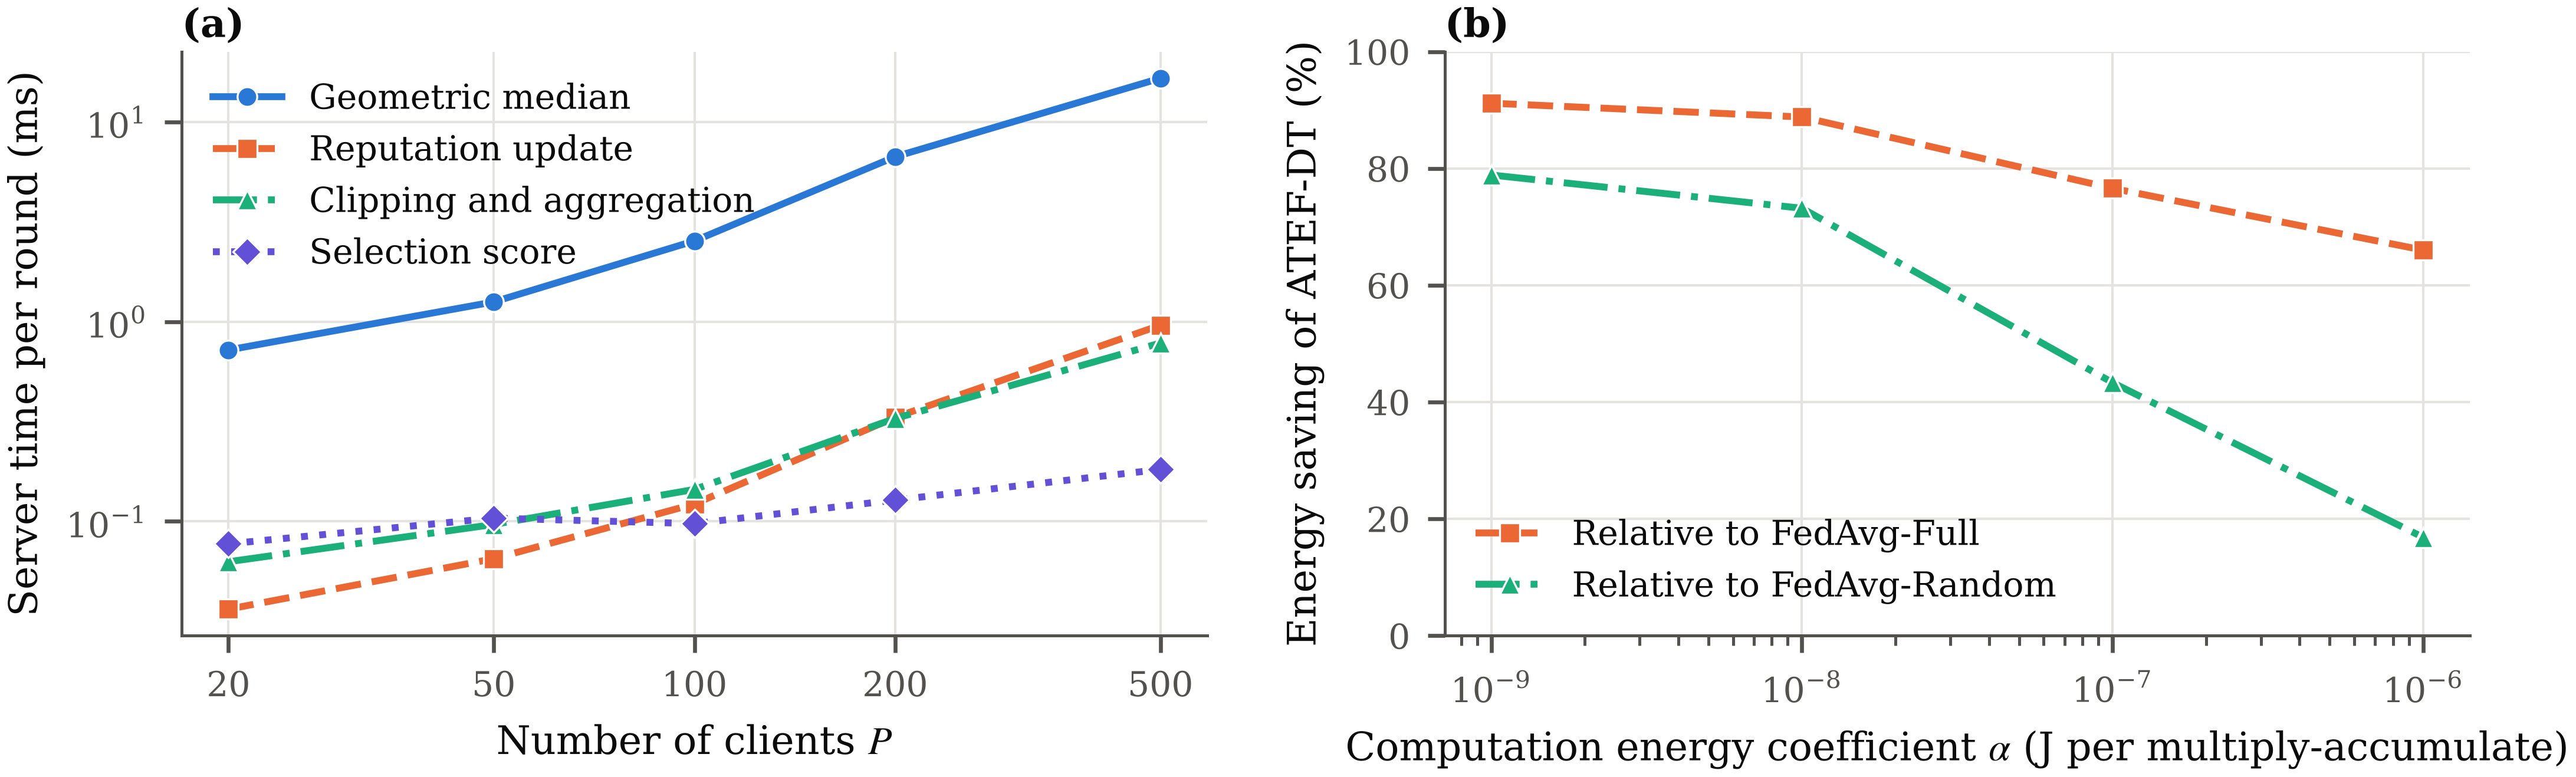
\includegraphics[width=\textwidth]{figures/fig_overhead}
	\revcap{R1.5, R2.5, R1.7(6)}{(a)~Server time per round and (b)~energy saving of ATEF-DT against the computation coefficient $\alpha$.}
	\label{fig:overhead}
\end{figure*}

\rtag{E5}\rev{Table~\ref{tab:overhead} reports the measured server time per round of the released single-threaded NumPy implementation.} The total grows from \V{t-total-20}~ms at 20 clients to \V{t-total-500}~ms at \V{pmax} clients and is dominated by the geometric median, which needs 10 to 15 Weiszfeld iterations; scoring and selection remain below a fifth of a millisecond. Figure~\ref{fig:overhead}(a) plots the components.

\subsection{Sensitivity to the Energy Parameters}
\label{subsec:sensitivity}
\rtag{R1.5, R2.5}\begin{revblock}Because the energy is computed from a model, its conclusions depend on the parameters of the model. Table~\ref{tab:alpha} and Figure~\ref{fig:overhead}(b) vary the computation coefficient $\alpha$ from $10^{-9}$ to $10^{-6}$~J. At the default, computation is \V{compshare-a6}\% of the energy of FedAvg-Full and the saving of ATEF-DT relative to FedAvg-Random is \V{sav-rand-a6}\%. As $\alpha$ decreases, communication dominates, quantization matters more, and the saving rises to \V{sav-rand-a8}\% at $10^{-8}$~J and \V{sav-rand-a9}\% at $10^{-9}$~J. The ranking of the methods also changes: for $\alpha\le 10^{-7}$~J, ATEF-DT consumes less than EA-FL, which transmits at full precision. The saving reported in Section~\ref{subsec:energyres} is therefore specific to a computation-dominated setting and is the smallest of those observed. Varying the amplifier efficiency $\eta_{\mathrm{PA}}$ between $0.2$ and $0.5$ changes the saving relative to FedAvg-Random only between \V{sav-rand-eta05}\% and \V{sav-rand-eta02}\%.\end{revblock}

\begin{table*}[t]
	\centering
	\revcap{R1.5, R2.5, E4}{Sensitivity to the computation energy coefficient $\alpha$.}
	\label{tab:alpha}
	\footnotesize
	\begin{tabular*}{\linewidth}{@{\extracolsep{\fill}}ccccccccc}
		\toprule
		 & \textbf{Computation} & \multicolumn{4}{c}{\textbf{Device energy (J)}} & \multicolumn{2}{c}{\textbf{Saving of ATEF-DT (\%)}} & \textbf{Jain index} \\
		\cmidrule(lr){3-6}\cmidrule(lr){7-8}
		$\boldsymbol{\alpha}$ \textbf{(J)} & \textbf{share (\%)} & \textbf{FedAvg-Full} & \textbf{FedAvg-Random} & \textbf{EA-FL} & \textbf{ATEF-DT} & \textbf{vs.\ Full} & \textbf{vs.\ Random} & \textbf{of ATEF-DT} \\
		\midrule
		\tabin{tab_alpha}
		\bottomrule
	\end{tabular*}
\end{table*}
